% !TEX TS-program = xelatex
\documentclass[12pt,a4paper]{article}

%% ─── Font & Encoding ───────────────────────────────────────────────
\usepackage{fontspec}
\usepackage{xepersian}

% Persian font
\settextfont{XB Niloofar}
\setdigitfont{XB Niloofar}

% English / Latin font
\setlatintextfont{Times New Roman}

%% ─── Page Layout ───────────────────────────────────────────────────
\usepackage[top=2.5cm, bottom=2.5cm, right=2.5cm, left=2.5cm]{geometry}

%% ─── Packages ──────────────────────────────────────────────────────
\usepackage{amsmath,amssymb,amsthm}
\usepackage{graphicx}
\usepackage{booktabs}
\usepackage{enumitem}
\usepackage{hyperref}
\usepackage{xcolor}

\usepackage{fancyhdr}
\usepackage{float}

%% ─── Hyperref Config ───────────────────────────────────────────────
\hypersetup{
    colorlinks=true,
    linkcolor=blue!70!black,
    citecolor=green!50!black,
    urlcolor=blue!60!black,
    pdftitle={شبیه‌سازی پاندول معکوس با چرخ واکنشی},
    pdfauthor={محمدرضا ولیخانی}
}

%% ─── Header / Footer ───────────────────────────────────────────────
\pagestyle{fancy}
\fancyhf{}
\fancyhead[R]{\thepage}
\fancyhead[L]{شبیه‌سازی پاندول معکوس}
\renewcommand{\headrulewidth}{0.4pt}

%% ─── Section Styling ───────────────────────────────────────────────
\usepackage{titlesec}
\titleformat{\section}
  {\Large\bfseries}
  {\thesection}{1em}{}
\titleformat{\subsection}
  {\large\bfseries}
  {\thesubsection}{1em}{}

%% ─── Custom Commands ───────────────────────────────────────────────
\newcommand{\authorname}{محمدرضا ولیخانی}
\newcommand{\doctitle}{شبیه‌سازی پاندول معکوس با چرخ واکنشی}

%% ─── Document ──────────────────────────────────────────────────────
\begin{document}

% Title page
\begin{titlepage}
    \centering
    \vspace*{1cm}

    % University logo
    
\includegraphics[width=3.5cm]{images/iust-logo.png}\par

    \vspace{0.8cm}

    {\Large\bfseries دانشگاه علم و صنعت\par}

    \vspace{0.4cm}

    {\large دانشکده مهندسی برق گرایش کنترل\par}

    \vspace{1.5cm}

    {\Huge\bfseries \doctitle\par}

    \vspace{2cm}

    {\Large فربد یونس پور\par}

    \vspace{0.3cm}

    {\Large محمدرضا ولیخانی\par}

    \vspace{1.8cm}

	{\small استاد راهنما\par}

	\vspace{0.3cm}
    {\Large دکتر صفار\par}

    \vfill

    {\large مرداد ۱۴۰۵\par}

    \vspace{1cm}

\end{titlepage}

% Table of contents
\tableofcontents
\newpage

% Sections
\section{مدل ریاضی سیستم}
\label{sec:system-math}

در این بخش، مدل ریاضی کامل سیستم پاندول معکوس با چرخ واکنشی را استخراج می‌کنیم. این سیستم یک نمونه کلاسیک از مسائل کنترل غیرخطی است که در آن، پایداری پاندول از طریق گشتاور واکنشی ایجادشده توسط یک چرخ دوار تأمین می‌شود. مدل نهایی یک دستگاه معادلات دیفرانسیل معمولی مرتبه پنجم است که هم‌زمان دینامیک مکانیکی و الکتریکی سیستم را توصیف می‌کند.

\subsection{نگاه کلی به سیستم و متغیرهای حالت}

سیستم مورد بررسی شامل یک بازوی پاندول صلب است که در انتهای آن، یک چرخ واکنشی (فلایویل) نصب شده است. این چرخ از طریق یک موتور \LR{DC} و جعبه‌دنده به بازو متصل است. با شتاب‌دهی یا کاهش سرعت چرخ، گشتاور واکنشی به بدنه پاندول وارد می‌شود و امکان کنترل زاویه پاندول فراهم می‌گردد.

مدل کامل سیستم شامل دو زیرسیستم جفت‌شده است:

\begin{itemize}
    \item \textbf{زیرسیستم مکانیکی:} بازوی پاندول و چرخ واکنشی، توصیف‌شده با یک ماتریس اینرسی کوپل $2 \times 2$.
    \item \textbf{زیرسیستم الکتریکی:} مدار آرمیچر موتور \LR{DC} شامل مقاومت، سلف‌گذاری و نیروی ضد محرکه الکتریکی (بک-\LR{EMF}).
\end{itemize}

بردار حالت سیستم به صورت زیر تعریف می‌شود:

\begin{equation}
    \mathbf{x} = \begin{bmatrix} \theta & \dot{\theta} & \varphi & \dot{\varphi} & i_a \end{bmatrix}^\top
\end{equation}

\noindent که در آن:

\begin{table}[H]
\centering
\begin{tabular}{lll}
\toprule
\textbf{متغیر} & \textbf{نماد} & \textbf{توضیح} \\
\midrule
زاویه پاندول & $\theta$ & زاویه نسبت به وضعیت عمودی ($\theta = 0$ در حالت عمودی) \\
سرعت زاویه‌ای پاندول & $\dot{\theta}$ & نرخ تغییرات $\theta$ \\
زاویه چرخ & $\varphi$ & زاویه چرخ نسبت به بازوی پاندول \\
سرعت زاویه‌ای چرخ & $\dot{\varphi}$ & نرخ تغییرات $\varphi$ (نسبی) \\
جریان آرمیچر & $i_a$ & جریان مدار آرمیچر موتور \\
\bottomrule
\end{tabular}
\end{table}

\subsection{پارامترهای فیزیکی}

پارامترهای سیستم در چهار گروه دسته‌بندی می‌شوند. مقادیر پیش‌فرض در جدول‌های زیر آمده است.

\subsubsection{پارامترهای پاندول}

\begin{table}[H]
\centering
\begin{tabular}{llcc}
\toprule
\textbf{پارامتر} & \textbf{نماد} & \textbf{مقدار پیش‌فرض} & \textbf{واحد} \\
\midrule
جرم پاندول & $m_p$ & $0.4$ & \LR{kg} \\
طول پاندول & $L_p$ & $0.3$ & \LR{m} \\
فاصله مرکز جرم از محور & $l_{cm}$ & $L_p / 2$ & \LR{m} \\
ممان اینرسی حول محور & $I_p$ & $\frac{1}{3} m_p L_p^2$ & \LR{kg·m²} \\
ضریب میرایی محور & $b$ & $0.001$ & \LR{N·m·s/rad} \\
\bottomrule
\end{tabular}
\end{table}

\subsubsection{پارامترهای چرخ واکنشی}

\begin{table}[H]
\centering
\begin{tabular}{llcc}
\toprule
\textbf{پارامتر} & \textbf{نماد} & \textbf{مقدار پیش‌فرض} & \textbf{واحد} \\
\midrule
جرم چرخ & $m_w$ & $0.25$ & \LR{kg} \\
شعاع داخلی چرخ & $r_i$ & $0.02$ & \LR{m} \\
شعاع خارجی چرخ & $r_o$ & $0.07$ & \LR{m} \\
ممان اینرسی چرخ & $I_w$ & $\frac{1}{2} m_w(r_o^2 + r_i^2)$ & \LR{kg·m²} \\
میرایی چرخ & $b_w$ & $0.0005$ & \LR{N·m·s/rad} \\
\bottomrule
\end{tabular}
\end{table}

\subsubsection{پارامترهای موتور و جعبه‌دنده}

\begin{table}[H]
\centering
\begin{tabular}{llcc}
\toprule
\textbf{پارامتر} & \textbf{نماد} & \textbf{مقدار پیش‌فرض} & \textbf{واحد} \\
\midrule
نسبت تبدیل جعبه‌دنده & $N$ & $4.0$ & --- \\
ثابت گشتاور / بک-\LR{EMF} & $K_t = K_e$ & $0.0876$ & \LR{N·m/A = V·s/rad} \\
مقاومت آرمیچر & $R_a$ & $1.2$ & $\Omega$ \\
سلف‌گذاری آرمیچر & $L_a$ & $0.0005$ & \LR{H} \\
ممان اینرسی روتور & $J_r$ & $5 \times 10^{-5}$ & \LR{kg·m²} \\
اصطکاک ویسکوز موتور & $b_m$ & $0.001$ & \LR{N·m·s/rad} \\
حداکثر ولتاژ & $V_{max}$ & $12.0$ & \LR{V} \\
\bottomrule
\end{tabular}
\end{table}

\subsubsection{پارامترهای محیطی و عددی}

\begin{table}[H]
\centering
\begin{tabular}{llcc}
\toprule
\textbf{پارامتر} & \textbf{نماد} & \textbf{مقدار پیش‌فرض} & \textbf{واحد} \\
\midrule
شتاب گرانش & $g$ & $9.81$ & \LR{m/s²} \\
گام زمانی انتگرال‌گیری & $\Delta t$ & $0.001$ & \LR{s} \\
\bottomrule
\end{tabular}
\end{table}

\subsection{کمیت‌های مشتق‌شده}

پیش از استخراج معادلات حرکت، چند کمیت مشتق‌شده را تعریف می‌کنیم که نقش محوری در ساده‌سازی روابط دارند.

\subsubsection{اینرسی مؤثر سمت چرخ}

ممان اینرسی روتور موتور از طریق جعبه‌دنده به سمت چرخ بازتاب داده می‌شود:

\begin{equation}
    I_{w,\text{eff}} = I_w + J_r \, N^2
\end{equation}

\subsubsection{میرایی مؤثر سمت چرخ}

به طور مشابه، اصطکاک ویسکوز موتور نیز به سمت چرخ منتقل می‌شود:

\begin{equation}
    b_{w,\text{eff}} = b_w + b_m \, N^2
\end{equation}

\subsubsection{ماتریس اینرسی کوپل}

ماتریس اینرسی $2 \times 2$ برای مختصات تعمیم‌یافته $(\theta, \varphi)$ به صورت زیر است:

\begin{equation}
    \mathbf{M} = \begin{bmatrix} M_{11} & M_{12} \\ M_{12} & M_{22} \end{bmatrix}
\end{equation}

\noindent که درایه‌های آن عبارتند از:

\begin{align}
    M_{11} &= I_p + m_w L_p^2 + I_{w,\text{eff}} \\
    M_{12} &= I_{w,\text{eff}} \\
    M_{22} &= I_{w,\text{eff}}
\end{align}

دترمینان این ماتریس برابر است با:

\begin{equation}
    \det(\mathbf{M}) = M_{11} M_{22} - M_{12}^2 > 0
\end{equation}

این کمیت باید اکیداً مثبت باشد تا سیستم از نظر فیزیکی معتبر باقی بماند.

\subsubsection{ضریب گرانشی}

ضریب گشتاور گرانشی ترکیبی به صورت زیر تعریف می‌شود:

\begin{equation}
    G = (m_p \, l_{cm} + m_w \, L_p) \, g
\end{equation}

این ضریب، اثر هم‌زمان جرم پاندول و جرم چرخ را در گشتاور گرانشی حول محور خلاصه می‌کند.

\subsection{معادلات حرکت}

\subsubsection{دینامیک مکانیکی (سیستم کوپل $2 \times 2$)}

معادلات حرکت مکانیکی از مکانیک لاگرانژی استخراج می‌شوند. موتور گشتاور الکترومغناطیسی $\tau_m = K_t \, i_a$ تولید می‌کند که از طریق جعبه‌دنده به صورت $\tau_w = N \, K_t \, i_a$ به چرخ منتقل می‌شود.

دستگاه معادلات به شکل ماتریسی زیر نوشته می‌شود:

\begin{equation}
    \mathbf{M} \begin{bmatrix} \ddot{\theta} \\ \ddot{\varphi} \end{bmatrix} = \begin{bmatrix} f_1 \\ f_2 \end{bmatrix}
\end{equation}

\noindent که در آن، نیروهای سمت راست برابرند با:

\begin{align}
    f_1 &= G \sin\theta - \tau_w - b\,\dot{\theta} + \tau_{\text{ext}} \\
    f_2 &= \tau_w - b_{w,\text{eff}} \, \dot{\varphi}
\end{align}

در این روابط، $\tau_{\text{ext}}$ گشتاور اغتشاش خارجی است که به بدنه پاندول اعمال می‌شود.

با استفاده از قاعده کرامر، شتاب‌های زاویه‌ای به دست می‌آیند:

\begin{align}
    \ddot{\theta} &= \frac{M_{22}\, f_1 - M_{12}\, f_2}{\det(\mathbf{M})} \\[6pt]
    \ddot{\varphi} &= \frac{M_{11}\, f_2 - M_{12}\, f_1}{\det(\mathbf{M})}
\end{align}

این روابط نشان می‌دهند که شتاب پاندول و شتاب چرخ به دلیل وجود درایه‌های غیرقطری $M_{12}$، به یکدیگر کوپل هستند. به بیان دیگر، اعمال گشتاور به چرخ، هم‌زمان بر حرکت پاندول و چرخ اثر می‌گذارد.

\subsubsection{دینامیک الکتریکی (مدار آرمیچر)}

مدار آرمیچر موتور \LR{DC} از قانون ولتاژ کیریشهف پیروی می‌کند:

\begin{equation}
    L_a \frac{di_a}{dt} = V - R_a\, i_a - K_e \, N \, \dot{\varphi}
\end{equation}

\noindent که در آن:
\begin{itemize}
    \item $V$ ولتاژ اعمال‌شده به آرمیچر است (محدودشده به بازه $[-V_{max},\, V_{max}]$)،
    \item $R_a\, i_a$ افت ولتاژ مقاومتی است،
    \item $K_e \, N \, \dot{\varphi}$ بک-\LR{EMF} است که متناسب با سرعت چرخ از طریق جعبه‌دنده می‌باشد.
\end{itemize}

بنابراین:

\begin{equation}
    \frac{di_a}{dt} = \frac{V - R_a\, i_a - K_e \, N \, \dot{\varphi}}{L_a}
\end{equation}

\subsubsection{فرم کامل فضای حالت}

با ترکیب معادلات مکانیکی و الکتریکی، مشتق بردار حالت پنج‌بعدی به صورت زیر نوشته می‌شود:

\begin{equation}
    \dot{\mathbf{x}} = \begin{bmatrix} \dot{\theta} \\ \ddot{\theta} \\ \dot{\varphi} \\ \ddot{\varphi} \\ \dot{i}_a \end{bmatrix}
    = \begin{bmatrix}
        x_2 \\[4pt]
        \dfrac{M_{22}\, f_1 - M_{12}\, f_2}{\det(\mathbf{M})} \\[8pt]
        x_4 \\[4pt]
        \dfrac{M_{11}\, f_2 - M_{12}\, f_1}{\det(\mathbf{M})} \\[8pt]
        \dfrac{V - R_a\, x_5 - K_e N\, x_4}{L_a}
    \end{bmatrix}
\end{equation}

\noindent با:

\begin{align}
    f_1 &= G \sin(x_1) - N K_t\, x_5 - b\, x_2 + \tau_{\text{ext}} \\
    f_2 &= N K_t\, x_5 - b_{w,\text{eff}}\, x_4
\end{align}

این دستگاه، مدل کامل غیرخطی سیستم را تشکیل می‌دهد و مبنای شبیه‌سازی عددی در گام‌های بعدی قرار می‌گیرد.

\subsection{انتگرال‌گیری عددی — روش رونگه‌کوتای مرتبه پنجم}

برای انتگرال‌گیری عددی دستگاه معادلات فوق، از روش رونگه‌کوتای شش‌مرحله‌ای مرتبه پنجم (بوتچر) استفاده می‌شود. این روش در مقایسه با روش کلاسیک \LR{RK4}، دقت بالاتر و پایستگی انرژی بهتری در بازه‌های زمانی طولانی ارائه می‌دهد.

\subsubsection{جدول بوتچر}

\begin{equation}
    \begin{array}{c|cccccc}
    0 & & & & & & \\
    \frac{1}{4} & \frac{1}{4} & & & & & \\
    \frac{1}{4} & \frac{1}{8} & \frac{1}{8} & & & & \\
    \frac{1}{2} & 0 & -\frac{1}{2} & 1 & & & \\
    \frac{3}{4} & \frac{3}{16} & 0 & 0 & \frac{9}{16} & & \\
    1 & -\frac{3}{7} & \frac{2}{7} & \frac{12}{7} & -\frac{12}{7} & \frac{8}{7} & \\
    \hline
    & \frac{7}{90} & 0 & \frac{32}{90} & \frac{12}{90} & \frac{32}{90} & \frac{7}{90}
    \end{array}
\end{equation}

\subsubsection{الگوریتم گام}

با فرض حالت $\mathbf{x}_n$ در زمان $t_n$ و گام $h = \Delta t$، شش مرحله به صورت زیر محاسبه می‌شوند:

\begin{align}
    \mathbf{k}_1 &= f(\mathbf{x}_n,\; V) \\
    \mathbf{k}_2 &= f\!\left(\mathbf{x}_n + \tfrac{h}{4}\mathbf{k}_1,\; V\right) \\
    \mathbf{k}_3 &= f\!\left(\mathbf{x}_n + \tfrac{h}{8}(\mathbf{k}_1 + \mathbf{k}_2),\; V\right) \\
    \mathbf{k}_4 &= f\!\left(\mathbf{x}_n + h(-\tfrac{1}{2}\mathbf{k}_2 + \mathbf{k}_3),\; V\right) \\
    \mathbf{k}_5 &= f\!\left(\mathbf{x}_n + h(\tfrac{3}{16}\mathbf{k}_1 + \tfrac{9}{16}\mathbf{k}_4),\; V\right) \\
    \mathbf{k}_6 &= f\!\left(\mathbf{x}_n + h(-\tfrac{3}{7}\mathbf{k}_1 + \tfrac{2}{7}\mathbf{k}_2 + \tfrac{12}{7}\mathbf{k}_3 - \tfrac{12}{7}\mathbf{k}_4 + \tfrac{8}{7}\mathbf{k}_5),\; V\right)
\end{align}

به‌روزرسانی حالت:

\begin{equation}
    \mathbf{x}_{n+1} = \mathbf{x}_n + \frac{h}{90}\left(7\mathbf{k}_1 + 32\mathbf{k}_3 + 12\mathbf{k}_4 + 32\mathbf{k}_5 + 7\mathbf{k}_6\right)
\end{equation}

پس از هر گام، زوایای $\theta$ و $\varphi$ به بازه $(-\pi,\, \pi]$ محدود می‌شوند.

\subsubsection{نکات پیاده‌سازی}

در پیاده‌سازی عددی، بافرهای شش مرحله ($\mathbf{k}_1$ تا $\mathbf{k}_6$) و یک بافر موقت، از پیش تخصیص داده می‌شوند تا از تخصیص حافظه در هر گام جلوگیری شود. تابع دینامیک نتایج را مستقیماً در آرایه خروجی از پیش تخصیص‌یافته می‌نویسد و ولتاژ پیش از ورود به انتگرال‌گیر به بازه $[-V_{max},\, V_{max}]$ محدود می‌شود.

\subsection{محاسبات انرژی}

\subsubsection{انرژی جنبشی}

\begin{equation}
    T = \frac{1}{2} \begin{bmatrix} \dot{\theta} & \dot{\varphi} \end{bmatrix} \mathbf{M} \begin{bmatrix} \dot{\theta} \\ \dot{\varphi} \end{bmatrix}
    = \frac{1}{2}\left(M_{11}\dot{\theta}^2 + 2M_{12}\dot{\theta}\dot{\varphi} + M_{22}\dot{\varphi}^2\right)
\end{equation}

\subsubsection{انرژی پتانسیل}

انرژی پتانسیل نسبت به وضعیت عمودی ($\theta = 0$) مرجع‌دهی می‌شود:

\begin{equation}
    U = G(\cos\theta - 1)
\end{equation}

در وضعیت عمودی $U = 0$ و در پایین‌تر از آن $U < 0$ است.

\subsubsection{انرژی مکانیکی کل}

\begin{equation}
    E = T + U
\end{equation}

\subsubsection{تکانه زاویه‌ای}

تکانه زاویه‌ای کل حول محور:

\begin{equation}
    \mathcal{L} = M_{11}\dot{\theta} + M_{12}\dot{\varphi}
\end{equation}

\subsection{کنترلرها}

تمام کنترلرها یک فرمان ولتاژ $V \in [-V_{\max},\, V_{\max}]$ تولید می‌کنند. فیزیک موتور و جعبه‌دنده به‌صورت داخلی این ولتاژ را از طریق دینامیک آرمیچر به گشتاور چرخ تبدیل می‌کند و کنترلرها هرگز مستقیماً گشتاور محاسبه نمی‌کنند.

دسته‌بندی کنترلرهای موجود در این پروژه عبارت است از:

\begin{itemize}
    \item \textbf{کنترلر \LR{PID}}: کنترلر کلاسیک بالانس با بهره‌های تناسبی، انتگرالی و مشتقی.
    \item \textbf{کنترلر \LR{LQR}}: تنظیم‌کننده خطی-درجه‌دو بر پایه مدل خطی‌شده چهارحالته شامل دینامیک الکتریکی.
    \item \textbf{بالاآوردن انرژی}: استراتژی آستروم--فوروتا مبتنی بر پمپاژ انرژی پاندول تا رسیدن به ناحیه عمودی.
    \item \textbf{بالاآوردن با خطی‌سازی بازخورد جزئی (\LR{PFL})}: شکل‌دهی شتاب مطلوب پاندول از طریق معکوس‌سازی دینامیک کوپل‌شده.
    \item \textbf{بالاآوردن ضربه‌ای سرعت‌صفر}: اعمال پالس ولتاژ در عبورهای صفر سرعت پاندول.
    \item \textbf{کنترلر مد لغزشی (\LR{SMC})}: کنترلر مقاوم با هموارسازی لایه مرزی برای کاهش چترینگ.
\end{itemize}

توضیحات دقیق، روابط ریاضی و جزئیات طراحی کنترلرهای بالانس در بخش~\ref{sec:controllers} و الگوریتم‌های بالاآوردن در بخش ۳ ارائه شده است.

\subsection{مدل اغتشاش}

اغتشاش‌های خارجی به دو شکل قابل اعمال هستند:

\begin{itemize}
    \item \textbf{کانال گشتاور:} گشتاور افزایشی $\tau_{\text{ext}}$ بر بدنه پاندول (وارد $f_1$ می‌شود).
    \item \textbf{کانال ولتاژ:} آفست ولتاژ افزایشی بر فرمان موتور.
\end{itemize}

شکل‌موج‌های پشتیبانی‌شده: ثابت، سینوسی، پالس، دندانه‌ارّه‌ای و نویز گاوسی.

\subsection{خروجی‌های تله‌متری}

در هر گام فیزیکی، کمیت‌های زیر برای تله‌متری محاسبه می‌شوند:

\begin{table}[h]
\centering
\begin{tabular}{ll}
\toprule
\textbf{کمیت} & \textbf{رابطه} \\
\midrule
بک-\LR{EMF} & $K_e \, N \, \dot{\varphi}$ \\
گشتاور موتور & $K_t \, i_a$ \\
گشتاور چرخ & $N \, K_t \, i_a$ \\
انرژی جنبشی & $\frac{1}{2}(M_{11}\dot{\theta}^2 + 2M_{12}\dot{\theta}\dot{\varphi} + M_{22}\dot{\varphi}^2)$ \\
انرژی پتانسیل & $G(\cos\theta - 1)$ \\
تکانه زاویه‌ای & $M_{11}\dot{\theta} + M_{12}\dot{\varphi}$ \\
\bottomrule
\end{tabular}
\end{table}

\subsection{محدودسازی زاویه}

پس از هر گام انتگرال‌گیری، زوایای $\theta$ و $\varphi$ به بازه $(-\pi,\, \pi]$ محدود می‌شوند:

\begin{equation}
    \alpha_{\text{wrapped}} = \left((\alpha + \pi) \mod 2\pi\right) - \pi
\end{equation}

این عملیات از رشد نامحدود زاویه جلوگیری می‌کند و هم‌زمان حالت فیزیکی سیستم را حفظ می‌نماید.

\subsection{جمع‌بندی}

سیستم پاندول معکوس با چرخ واکنشی، یک سیستم الکترومکانیکی پنج‌حالته است که شامل موارد زیر می‌شود:

\begin{enumerate}
    \item مکانیک اجسام صلب کوپل‌شده (ماتریس اینرسی $2 \times 2$ برای پاندول و چرخ)،
    \item دینامیک الکتریکی موتور \LR{DC} (مدار آرمیچر با بک-\LR{EMF})،
    \item انتقال جعبه‌دنده (بازتاب اینرسی روتور و اصطکاک به سمت چرخ)،
    \item چندین استراتژی کنترل (\LR{PID}، \LR{LQR}، بالاآوردن انرژی، \LR{PFL}، مد لغزشی).
\end{enumerate}

انتگرال‌گیری عددی با روش رونگه‌کوتای مرتبه پنجم و در فرکانس $1$ کیلوهرتز انجام می‌شود که دقت مناسب و پایداری عددی لازم برای شبیه‌سازی بلادرنگ تعاملی را فراهم می‌آورد.
\newpage
\section{روش‌های کنترل}
\label{sec:controllers}

در این بخش، روش‌های کنترل پیاده‌سازی‌شده برای پایدارسازی پاندول معکوس با چرخ واکنشی را معرفی می‌کنیم. تمامی کنترلرها یک فرمان \textbf{ولتاژ} $V$ به مدار آرمیچر موتور DC اعمال می‌کنند. ولتاژ خروجی همواره در محدوده مجاز اشباع می‌شود:

\begin{equation}
V_{\text{applied}} = \operatorname{clip}(V,\; -V_{\max},\; V_{\max})
\end{equation}

این محدودیت، رفتار واقعی عملگر الکتریکی را منعکس می‌کند؛ زیرا ولتاژ قابل اعمال به آرمیچر در عمل محدود است.

پیش از معرفی کنترلرها، یادآوری می‌کنیم که بردار حالت سیستم به صورت زیر تعریف شده است:

\begin{equation}
\mathbf{x} = \begin{bmatrix} \theta & \dot{\theta} & \varphi & \dot{\varphi} & i_a \end{bmatrix}^\top
\end{equation}

که در آن $\theta$ زاویه پاندول، $\varphi$ زاویه چرخ واکنشی و $i_a$ جریان آرمیچر است. دینامیک مکانیکی سیستم از ماتریس اینرسی کوپل‌شده $2 \times 2$ و دینامیک الکتریکی از معادله مدار آرمیچر به‌دست می‌آید. کنترلرها مستقیماً گشتاور محاسبه نمی‌کنند؛ بلکه ولتاژ ورودی را مشخص می‌کنند و فیزیک موتور (اتصال مستقیم، $N=1$) به‌صورت داخلی در شبیه‌ساز، ولتاژ را به گشتاور چرخ تبدیل می‌کند.

% ─────────────────────────────────────────────────────────────────────
\subsection{بدون کنترل}

ساده‌ترین حالت ممکن، اعمال ولتاژ صفر است:

\begin{equation}
V = 0
\end{equation}

در این حالت، پاندول تنها تحت اثر گرانش و میرایی حرکت می‌کند و هیچ نیروی اصلاحی اعمال نمی‌شود. از آنجا که نقطه تعادل عمودی پاندول معکوس ناپایدار است، سیستم در این حالت از تعادل خارج شده و سقوط می‌کند. این حالت برای مشاهده پاسخ حلقه‌باز سیستم و مقایسه عملکرد کنترلرها مفید است.

شکل~\ref{fig:open-loop} پاسخ حلقه‌باز پاندول را از زاویه اولیه $\theta_0 = 0.1$ رادیان بدون اعمال هیچ فرمان کنترلی نشان می‌دهد. همان‌طور که انتظار می‌رود، پاندول تحت اثر گشتاور گرانشی از وضعیت عمودی فاصله گرفته و سقوط می‌کند.

\begin{figure}[H]
\centering
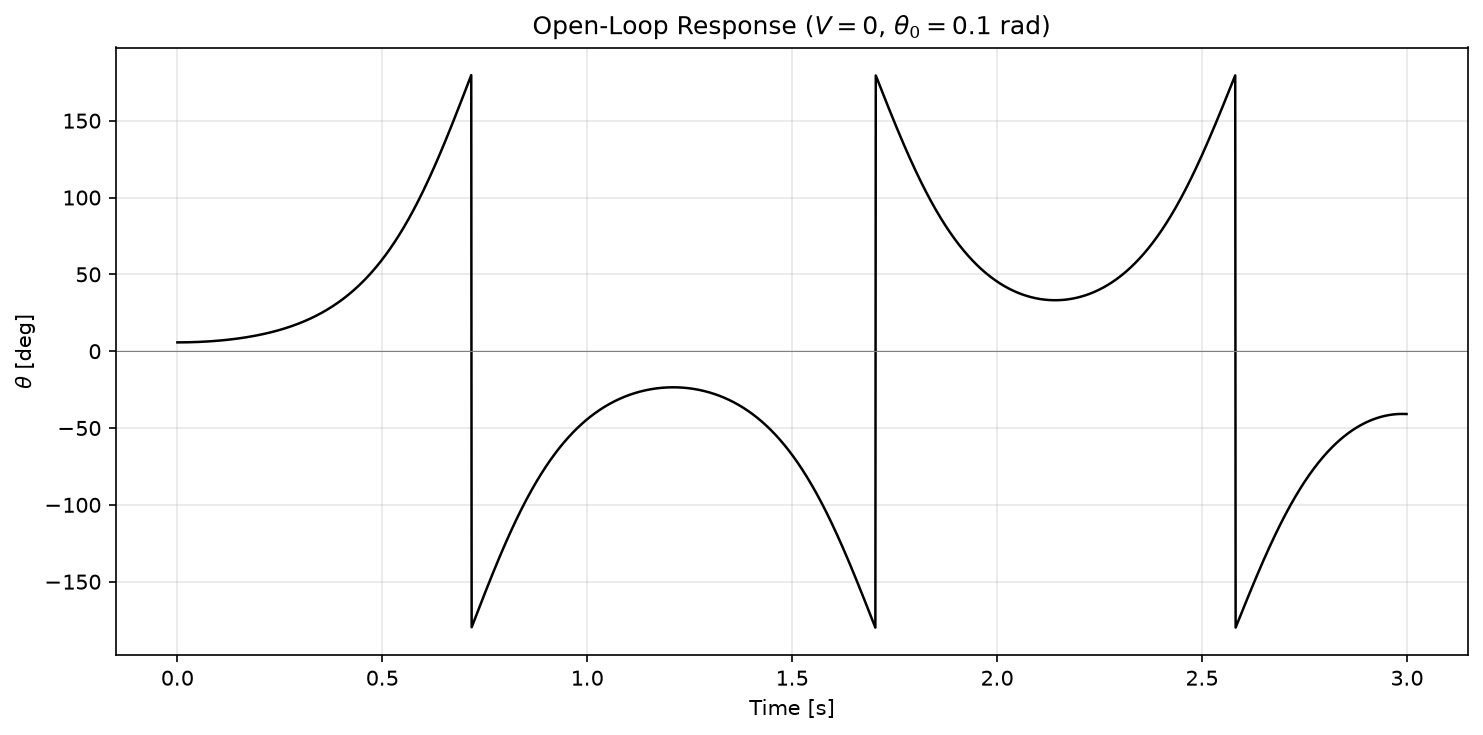
\includegraphics[width=0.85\textwidth]{results/open_loop_response.png}
\caption{پاسخ حلقه‌باز پاندول معکوس بدون کنترل ($\theta_0 = 0.1$ رادیان)}
\label{fig:open-loop}
\end{figure}

% ─────────────────────────────────────────────────────────────────────
\subsection{کنترل دستی}

در حالت کنترل دستی، کاربر یک ولتاژ ثابت $V_{\text{set}}$ را مشخص می‌کند و این ولتاژ پس از اعمال محدودیت اشباع به آرمیچر فرستاده می‌شود:

\begin{equation}
V = \operatorname{clip}(V_{\text{set}},\; -V_{\max},\; V_{\max})
\end{equation}

در این حالت هیچ بازخوردی از وضعیت سیستم وجود ندارد. کاربرد اصلی این حالت، آزمایش‌های حلقه‌باز و شناسایی رفتار سیستم است.

% ─────────────────────────────────────────────────────────────────────
\subsection{کنترلر PID}

\subsubsection{قانون کنترل}

کنترلر PID زاویه پاندول $\theta$ را حول نقطه تعادل عمودی ($\theta = 0$) تنظیم می‌کند. سیگنال کنترلی به صورت زیر محاسبه می‌شود:

\begin{equation}
V = K_p\, \theta + K_i \int_0^t \theta(\tau)\, d\tau + K_d\, \dot{\theta}
\end{equation}

هر یک از بهره‌ها نقش مشخصی در رفتار سیستم دارند:

\begin{itemize}[itemsep=2pt]
    \item $K_p$ (بهره تناسبی): اصلاح متناسب با خطای زاویه. افزایش این بهره سرعت پاسخ را بالا می‌برد، اما ممکن است باعث افزایش نوسان شود.
    \item $K_i$ (بهره انتگرالی): حذف خطای ماندگار. این جمله انحراف ثابت از نقطه تعادل را در طول زمان جبران می‌کند.
    \item $K_d$ (بهره مشتقی): میرایی متناسب با سرعت زاویه‌ای. این جمله نوسانات را کاهش می‌دهد و پایداری را بهبود می‌بخشد.
\end{itemize}

قرارداد علامت به این صورت است که زاویه مثبت $\theta$ نیازمند ولتاژ اصلاحی مثبت است.

\subsubsection{جلوگیری از اشباع انتگرال}

یکی از مشکلات رایج کنترلرهای PID در حضور محدودیت عملگر، پدیده باد کردن انتگرال (Integral Windup) است. هنگامی که خروجی کنترلر در اشباع قرار دارد، جمله انتگرالی به تجمع ادامه می‌دهد و پس از خروج از اشباع، باعث پاسخ بیش‌ازحد و تأخیر در بازیابی می‌شود.

برای مقابله با این پدیده، از روش توقف شرطی (Clamping) استفاده می‌کنیم. در هر گام زمانی با فاصله $\Delta t$، ابتدا خروجی آزمایشی محاسبه می‌شود:

\begin{equation}
u_{\text{trial}} = K_p\,\theta + K_i\,I + K_d\,\dot{\theta}
\end{equation}

که در آن $I$ مقدار تجمعی انتگرال است. قانون به‌روزرسانی انتگرال به صورت زیر است:

\begin{itemize}[itemsep=2pt]
    \item اگر $|u_{\text{trial}}| < V_{\max}$، انتگرال به‌صورت عادی به‌روز می‌شود:
    \begin{equation}
    I \leftarrow I + \theta\,\Delta t
    \end{equation}
    \item اگر $|u_{\text{trial}}| \ge V_{\max}$، انتگرال تنها در صورتی به‌روز می‌شود که تجمع آن در جهت کاهش اشباع باشد:
    \begin{equation}
    I \leftarrow I + \theta\,\Delta t \quad \text{if} \quad (u_{\text{trial}} > 0 \;\wedge\; \theta < 0) \;\;\vee\;\; (u_{\text{trial}} < 0 \;\wedge\; \theta > 0)
    \end{equation}
    \item در غیر این صورت، انتگرال ثابت نگه داشته می‌شود.
\end{itemize}

این مکانیزم از تجمع بی‌رویه جمله انتگرالی در دوران اشباع جلوگیری می‌کند و همزمان امکان بازیابی سریع پس از خروج از اشباع را حفظ می‌نماید.

\subsubsection{خروجی نهایی}

خروجی نهایی کنترلر PID با اعمال محدودیت ولتاژ به‌دست می‌آید:

\begin{equation}
V = \operatorname{clip}\!\big(K_p\,\theta + K_i\,I + K_d\,\dot{\theta},\; -V_{\max},\; V_{\max}\big)
\end{equation}

% ─────────────────────────────────────────────────────────────────────
\subsection{کنترلر LQR}

\subsubsection{خطی‌سازی}

کنترلر LQR بر اساس مدل خطی‌شده سیستم حول نقطه تعادل عمودی ($\theta = 0$) طراحی می‌شود. برخلاف کنترلر PID که تنها از دو حالت مکانیکی استفاده می‌کند، LQR از یک مدل \textbf{چهارحالته} بهره می‌برد که دینامیک الکتریکی آرمیچر را نیز شامل می‌شود:

\begin{equation}
\mathbf{x} = \begin{bmatrix} \theta & \dot{\theta} & \dot{\varphi} & i_a \end{bmatrix}^\top,
\qquad
u = V
\end{equation}

سیستم خطی‌شده به فرم فضاست حالت نوشته می‌شود:

\begin{equation}
\dot{\mathbf{x}} = \mathbf{A}\,\mathbf{x} + \mathbf{B}\,V
\end{equation}

\subsubsection{ماتریس‌های سیستم}

با تعریف $\Delta = M_{11} M_{22} - M_{12}^2$ به‌عنوان دترمینان ماتریس اینرسی، ماتریس $\mathbf{A}$ به صورت زیر به‌دست می‌آید:

\begin{equation}
\mathbf{A} = \begin{bmatrix}
0 & 1 & 0 & 0 \\[6pt]
\dfrac{M_{22}\,G}{\Delta}
& -\dfrac{M_{22}\,b}{\Delta}
& \dfrac{M_{12}\,b_{w,\text{eff}}}{\Delta}
& -\dfrac{(M_{22}+M_{12})\,N K_t}{\Delta} \\[10pt]
-\dfrac{M_{12}\,G}{\Delta}
& \dfrac{M_{12}\,b}{\Delta}
& -\dfrac{M_{11}\,b_{w,\text{eff}}}{\Delta}
& \dfrac{(M_{11}+M_{12})\,N K_t}{\Delta} \\[10pt]
0 & 0 & -\dfrac{K_e N}{L_a} & -\dfrac{R_a}{L_a}
\end{bmatrix}
\end{equation}

بردار ورودی $\mathbf{B}$ نشان می‌دهد که ولتاژ تنها در معادله الکتریکی وارد می‌شود:

\begin{equation}
\mathbf{B} = \begin{bmatrix} 0 \\ 0 \\ 0 \\ 1/L_a \end{bmatrix}
\end{equation}

در این روابط، $G$ ضریب گرانش، $b$ ضریب میرایی پاندول، $b_{w,\text{eff}}$ میرایی مؤثر چرخ، $N$ نسبت جعبه‌دنده، $K_t$ ثابت گشتاور، $K_e$ ثابت نیروی ضد محرکه، $L_a$ سلف آرمیچر و $R_a$ مقاومت آرمیچر است.

با جایگذاری پارامترهای فیزیکی پیش‌فرض (جدول بخش~\ref{sec:system-math})، مقادیر عددی ماتریس‌ها به صورت زیر است:

\begin{equation}
\mathbf{A} = \begin{bmatrix}
0 & 1 & 0 & 0 \\
38.3870 & -0.0290 & 0.0435 & -5.0783 \\
-38.3870 & 0.0290 & -2.1488 & 128.0200 \\
0 & 0 & -175.2000 & -2400.0000
\end{bmatrix},
\qquad
\mathbf{B} = \begin{bmatrix} 0 \\ 0 \\ 0 \\ 2000.0000 \end{bmatrix}
\end{equation}

مقادیر بزرگ در سطر چهارم ماتریس $\mathbf{A}$ و بردار $\mathbf{B}$ بازتاب دینامیک سریع الکتریکی آرمیچر (ثابت زمانی $\tau_a = L_a/R_a \approx 0.42$ میلی‌ثانیه) هستند.

\subsubsection{مسئله بهینه‌سازی}

کنترلر LQR هزینه درجه‌دوم افق بی‌نهایت را کمینه می‌کند:

\begin{equation}
J = \int_0^\infty \!\big(\mathbf{x}^\top \mathbf{Q}\, \mathbf{x} + u^\top \mathbf{R}\, u\big)\, dt
\end{equation}

ماتریس‌های وزن به صورت زیر تعریف می‌شوند:

\begin{equation}
\mathbf{Q} = \operatorname{diag}(q_\theta,\; q_{\dot{\theta}},\; q_{\dot{\varphi}},\; q_{i_a}),
\qquad
\mathbf{R} = r
\end{equation}

هر وزن، اهمیت نسبی یک متغیر را در تابع هزینه مشخص می‌کند:

\begin{table}[H]
\centering
\caption{نقش وزن‌ها در تابع هزینه LQR}
\begin{tabular}{ll}
\toprule
\textbf{وزن} & \textbf{کمینه‌سازی} \\
\midrule
$q_\theta$ & انحراف زاویه از وضعیت عمودی \\
$q_{\dot{\theta}}$ & سرعت زاویه‌ای پاندول \\
$q_{\dot{\varphi}}$ & سرعت زاویه‌ای چرخ واکنشی \\
$q_{i_a}$ & جریان آرمیچر (تلاش الکتریکی) \\
$r$ & بزرگی ولتاژ کنترلی \\
\bottomrule
\end{tabular}
\end{table}

افزایش یک وزن نسبت به سایرین، اهمیت کاهش آن متغیر را بالا می‌برد و در نتیجه، کنترلر تلاش بیشتری برای محدود کردن آن صرف می‌کند.

\subsubsection{معادله ریکاتی و بهره بهینه}

بهره بهینه بازخورد حالت از حل معادله جبری ریکاتی پیوسته (CARE) به‌دست می‌آید:

\begin{equation}
\mathbf{A}^\top \mathbf{P} + \mathbf{P}\,\mathbf{A}
- \mathbf{P}\,\mathbf{B}\,\mathbf{R}^{-1}\,\mathbf{B}^\top\,\mathbf{P}
+ \mathbf{Q} = \mathbf{0}
\end{equation}

پس از محاسبه ماتریس متقارن مثبت معین $\mathbf{P}$، بردار بهره بهینه برابر است با:

\begin{equation}
\mathbf{K} = \mathbf{R}^{-1}\,\mathbf{B}^\top\,\mathbf{P}
\end{equation}

\subsubsection{قانون کنترل}

فرمان ولتاژ نهایی از ضرب منفی بردار بهره در بردار حالت به‌دست می‌آید:

\begin{equation}
V = -\mathbf{K}\,\mathbf{x}
= -\big(k_1\,\theta + k_2\,\dot{\theta} + k_3\,\dot{\varphi} + k_4\, i_a\big)
\end{equation}

نتیجه در محدوده $[-V_{\max},\, V_{\max}]$ محدود می‌شود.

\subsubsection{محاسبه مجدد بهره و حالت جایگزین}

بهره $\mathbf{K}$ به‌صورت تنبل (Lazy) و تنها در صورت تغییر پارامترهای فیزیکی یا کنترلی بازمحاسبه می‌شود. این رویکرد از تکرار غیرضروری محاسبه پرهزینه ریکاتی در هر گام فیزیک جلوگیری می‌کند.

در صورتی که حل معادله ریکاتی ناموفق باشد (برای نمونه، دترمینان ماتریس اینرسی نامثبت یا بهره‌های غیرمتناهی)، کنترلر به‌صورت خودکار به رفتار PID بازمی‌گردد و یک هشدار ثبت می‌شود.

% ─────────────────────────────────────────────────────────────────────
\subsection{کنترلر مد لغزشی}

\subsubsection{سطح لغزشی}

در کنترل مد لغزشی (Sliding Mode Control)، یک سطح لغزشی اسکالر به‌عنوان ترکیب خطی از حالت‌های قابل اندازه‌گیری تعریف می‌شود:

\begin{equation}
s = c_1\,\theta + c_2\,\dot{\theta} + c_3\,\dot{\varphi}
\end{equation}

ضرایب $c_1$، $c_2$ و $c_3$ به‌ترتیب وزن خطای زاویه، سرعت پاندول و سرعت چرخ را مشخص می‌کنند. هدف طراحی، هدایت متغیر $s$ به سمت صفر است. هنگامی که $s = 0$، دینامیک سیستم بر روی یک منیفولد مطلوب محدود می‌شود.

\subsubsection{تابع اشباع لایه مرزی}

در کنترل مد لغزشی کلاسیک، از تابع علامت $\operatorname{sgn}(s)$ استفاده می‌شود. این تابع باعث پدیده چترینگ (Chattering) می‌شود؛ یعنی نوسانات فرکانس بالا حول سطح لغزشی که در عمل می‌تواند به عملگر آسیب برساند.

برای کاهش چترینگ، از تقریب لایه مرزی استفاده می‌کنیم. در این روش، تابع علامت با تابع اشباع جایگزین می‌شود:

\begin{equation}
\operatorname{sat}\!\left(\frac{s}{\Phi}\right) =
\begin{cases}
\dfrac{s}{\Phi} & \text{if } \left|\dfrac{s}{\Phi}\right| \le 1 \\[8pt]
\operatorname{sgn}(s) & \text{if } \left|\dfrac{s}{\Phi}\right| > 1
\end{cases}
\end{equation}

در این رابطه، $\Phi > 0$ ضخامت لایه مرزی است. درون لایه ($|s| \le \Phi$)، رفتار کنترلر خطی و هموار است. بیرون لایه، کنترلر مانند حالت سوئیچینگ کلاسیک عمل می‌کند. افزایش $\Phi$ چترینگ را بیشتر کاهش می‌دهد، اما دقت ردیابی را کاهش می‌دهد.

\subsubsection{قانون کنترل}

سیگنال کنترلی مد لغزشی به صورت زیر محاسبه می‌شود:

\begin{equation}
V = -K\,\operatorname{sat}\!\left(\frac{s}{\Phi}\right) - \eta\, s
\end{equation}

نقش هر پارامتر در جدول زیر آمده است:

\begin{table}[H]
\centering
\caption{پارامترهای کنترلر مد لغزشی}
\begin{tabular}{ll}
\toprule
\textbf{پارامتر} & \textbf{نقش} \\
\midrule
$K$ & بهره سوئیچینگ؛ هدایت حالت به سمت سطح لغزشی \\
$\eta$ & بهره تناسبی؛ ایجاد میرایی پیوسته روی سطح \\
$\Phi$ & ضخامت لایه مرزی؛ مصالحه بین کاهش چترینگ و دقت \\
\bottomrule
\end{tabular}
\end{table}

خروجی نهایی در محدوده $[-V_{\max},\, V_{\max}]$ محدود می‌شود.

\subsubsection{تحلیل پایداری}

برای بررسی پایداری، تابع لیاپانوف $\mathcal{V} = \tfrac{1}{2}s^2$ را در نظر می‌گیریم. بیرون از لایه مرزی، مشتق زمانی این تابع در شرط $\dot{\mathcal{V}} = s\,\dot{s} < 0$ صدق می‌کند. این شرط تضمین می‌کند که متغیر $s$ در زمان متناهی به لایه مرزی می‌رسد و خطای ردیابی در محدوده $O(\Phi)$ کراندار باقی می‌ماند.

شکل~\ref{fig:smc-step} پاسخ پله کنترلر مد لغزشی را با پارامترهای پیش‌فرض نشان می‌دهد. همان‌طور که مشاهده می‌شود، متغیر لغزشی $s$ در مدت کوتاهی به لایه مرزی وارد شده و زاویه پاندول به‌صورت همگرا به سمت صفر میل می‌کند.

\begin{figure}[H]
\centering
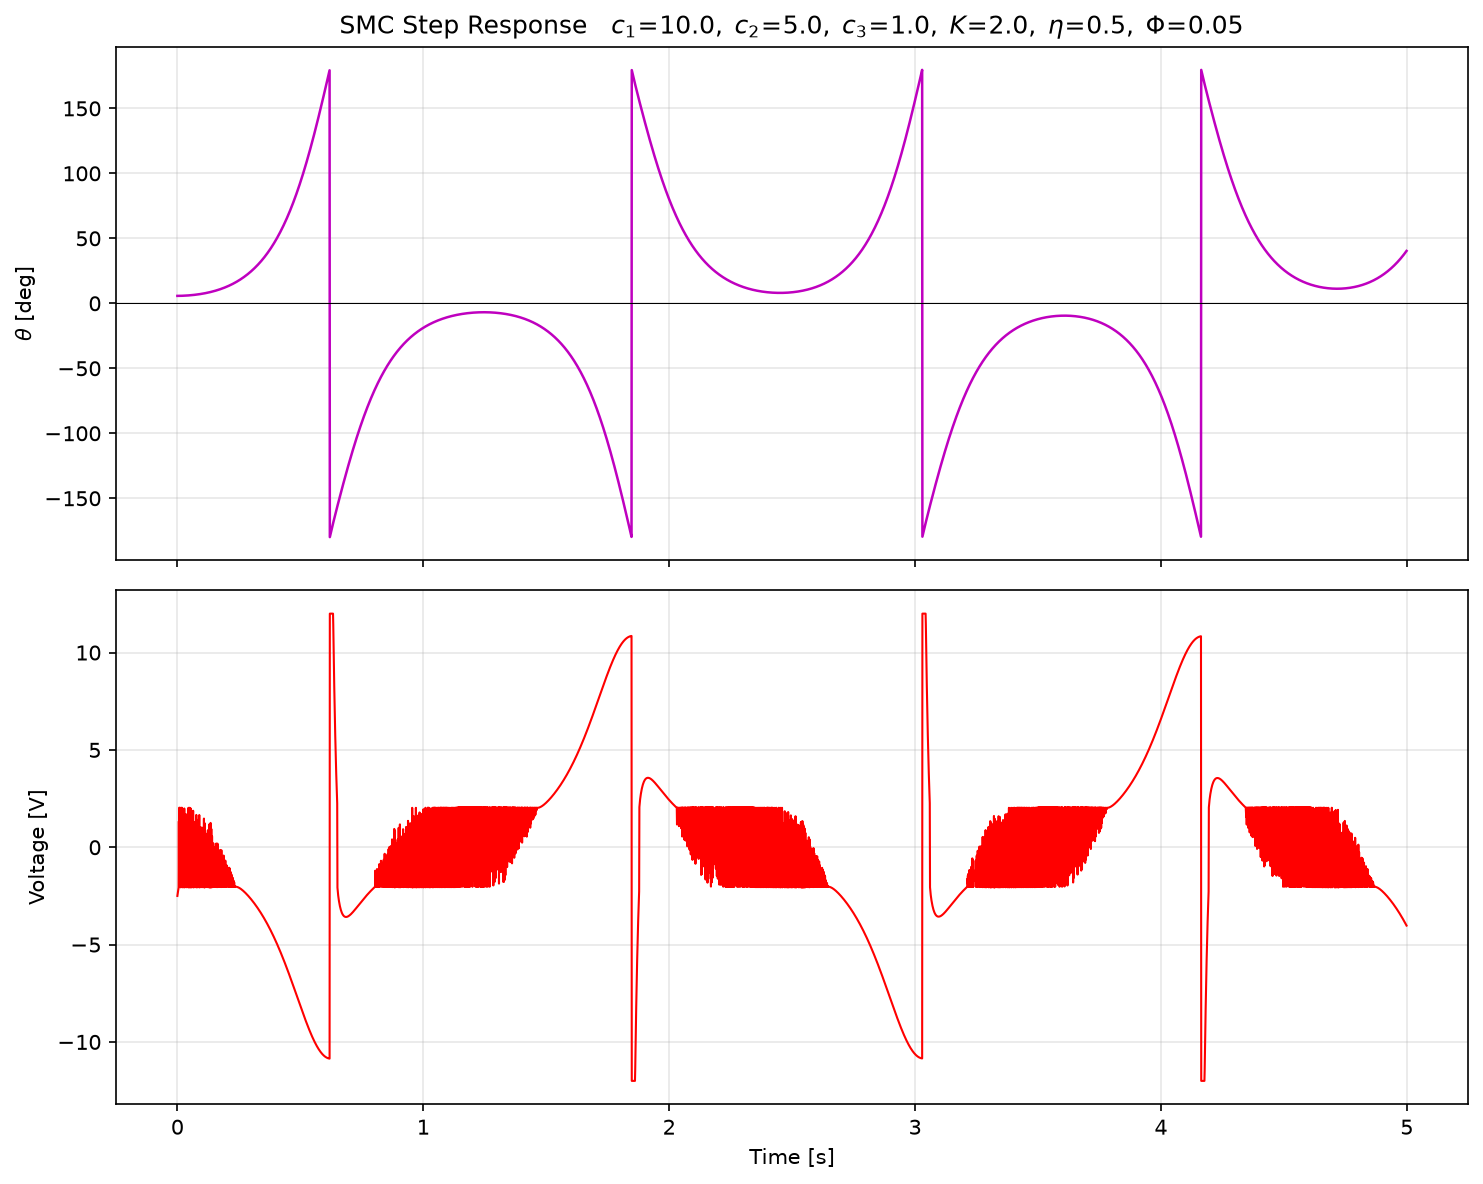
\includegraphics[width=0.85\textwidth]{results/smc_step_response.png}
\caption{پاسخ پله کنترلر مد لغزشی با لایه مرزی ($\theta_0 = 0.1$ رادیان)}
\label{fig:smc-step}
\end{figure}

% ─────────────────────────────────────────────────────────────────────
\subsection{مقایسه روش‌ها}

جدول زیر خلاصه‌ای از ویژگی‌های هر کنترلر را ارائه می‌دهد:

\begin{table}[H]
\centering
\caption{مقایسه روش‌های کنترل}
\begin{tabular}{llll}
\toprule
\textbf{کنترلر} & \textbf{حالت‌های استفاده‌شده} & \textbf{پارامترهای اصلی} & \textbf{خروجی} \\
\midrule
بدون کنترل & --- & --- & $V = 0$ \\
دستی & --- & $V_{\text{set}}$ & $V = V_{\text{set}}$ \\
PID & $\theta,\;\dot\theta$ & $K_p,\;K_i,\;K_d$ & $V = K_p\theta + K_i\!\int\theta + K_d\dot\theta$ \\
LQR & $\theta,\;\dot\theta,\;\dot\varphi,\;i_a$ & $\mathbf{Q},\;r$ & $V = -\mathbf{Kx}$ \\
مد لغزشی & $\theta,\;\dot\theta,\;\dot\varphi$ & $c_1,c_2,c_3,\;K,\;\eta,\;\Phi$ & $V = -K\,\text{sat}(s/\Phi) - \eta\,s$ \\
\bottomrule
\end{tabular}
\end{table}

شکل~\ref{fig:three-comparison} مقایسه هم‌زمان پاسخ پله سه کنترلر PID، LQR و مد لغزشی را نشان می‌دهد.

\begin{figure}[H]
\centering
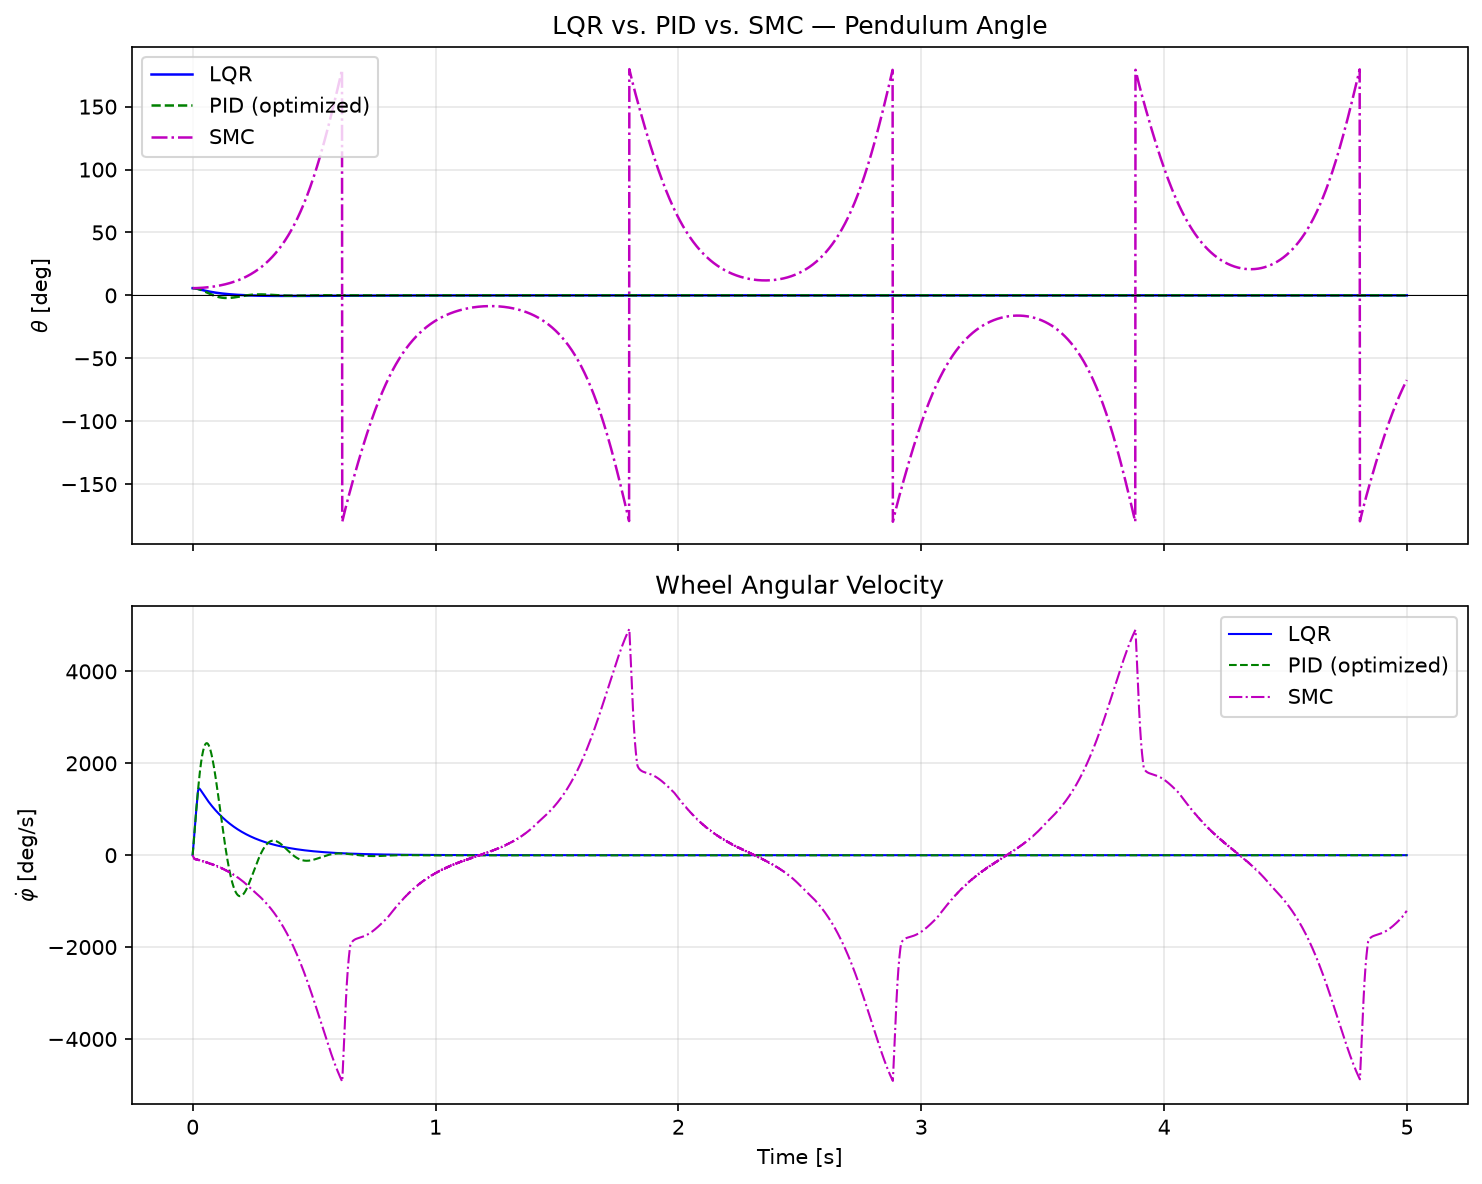
\includegraphics[width=0.85\textwidth]{results/three_controller_comparison.png}
\caption{مقایسه پاسخ پله کنترلرهای PID، LQR و مد لغزشی ($\theta_0 = 0.1$ رادیان)}
\label{fig:three-comparison}
\end{figure}

کنترلر LQR به دلیل استفاده از مدل کامل چهارحالته و بهینه‌سازی هم‌زمان، سریع‌ترین زمان نشست و کمترین نوسان را در میان سه روش دارد. کنترلر PID با ساختار ساده‌تر، پاسخ قابل‌قبولی ارائه می‌دهد، اما اندکی بیش‌جهت بیشتر و زمان نشست طولانی‌تری نسبت به LQR دارد. کنترلر مد لغزشی از نظر مقاومت در برابر عدم قطعیت پارامترها برتری دارد؛ هرچند به دلیل استفاده از لایه مرزی، همگرایی آن کمی هموارتر و با شیب ملایم‌تری نسبت به دو روش دیگر صورت می‌گیرد.

نکته مشترک تمامی روش‌ها این است که خروجی آن‌ها ولتاژ آرمیچر است. فیزیک موتور شامل نیروی ضد محرکه، سلف، مقاومت و نسبت تبدیل ($N=1$، اتصال مستقیم) به‌صورت داخلی در شبیه‌ساز رسیدگی می‌شود و کنترلرها هرگز مستقیماً گشتاور محاسبه نمی‌کنند.

از نظر عملکردی، کنترلر PID ساده‌ترین ساختار را دارد و برای سیستم‌هایی با دینامیک نسبتاً کند مناسب است. کنترلر LQR با استفاده از مدل کامل سیستم و بهینه‌سازی تابع هزینه، عملکرد بهتری در نزدیکی نقطه تعادل ارائه می‌دهد. کنترلر مد لغزشی در برابر عدم قطعیت پارامترها مقاوم‌تر است، اما طراحی آن نیازمند انتخاب دقیق ضخامت لایه مرزی برای مصالحه بین چترینگ و دقت است.

% ─────────────────────────────────────────────────────────────────────
\subsection{نتایج عددی تنظیم بهره}
\label{sec:gain-results}

در این بخش، نتایج عددی محاسبه بهره‌های بهینه برای کنترلرهای LQR و PID ارائه می‌شود. این مقادیر با استفاده از پارامترهای فیزیکی پیش‌فرض سیستم (جدول‌های بخش~\ref{sec:system-math}) و حل عددی معادله ریکاتی و بهینه‌سازی ITAE به‌دست آمده‌اند.

\subsubsection{بهره‌های بهینه LQR}

با انتخاب ماتریس‌های وزن زیر:

\begin{equation}
\mathbf{Q} = \operatorname{diag}(100,\; 1,\; 10,\; 0.01), \qquad r = 1.0
\end{equation}

حل معادله جبری ریکاتی با ماتریس‌های به‌روز‌شده ($N=1$)، بردار بهره بهینه زیر را تولید می‌کند:

\begin{equation}
\mathbf{K} = \begin{bmatrix} -844.46 & -138.69 & -2.32 & 0.16 \end{bmatrix}
\end{equation}

قطب‌های حلقه‌بسته سیستم با این بهره‌ها عبارتند از:

\begin{equation}
\lambda_1 \approx -2374.6, \quad \lambda_2 \approx -341.2, \quad \lambda_3 \approx -6.12, \quad \lambda_4 \approx -6.02
\end{equation}

دو قطب سریع ($\lambda_1$ و $\lambda_2$) مربوط به دینامیک الکتریکی آرمیچر هستند و دو قطب کندتر ($\lambda_3$ و $\lambda_4$) دینامیک مکانیکی پاندول را کنترل می‌کنند. قرارگیری تمام قطب‌ها در نیم‌صفحه چپ، پایداری مجانبی حلقه‌بسته را تضمین می‌کند.

شکل~\ref{fig:lqr-step} پاسخ پله کنترلر LQR را با این بهره‌ها نشان می‌دهد.

\begin{figure}[H]
\centering
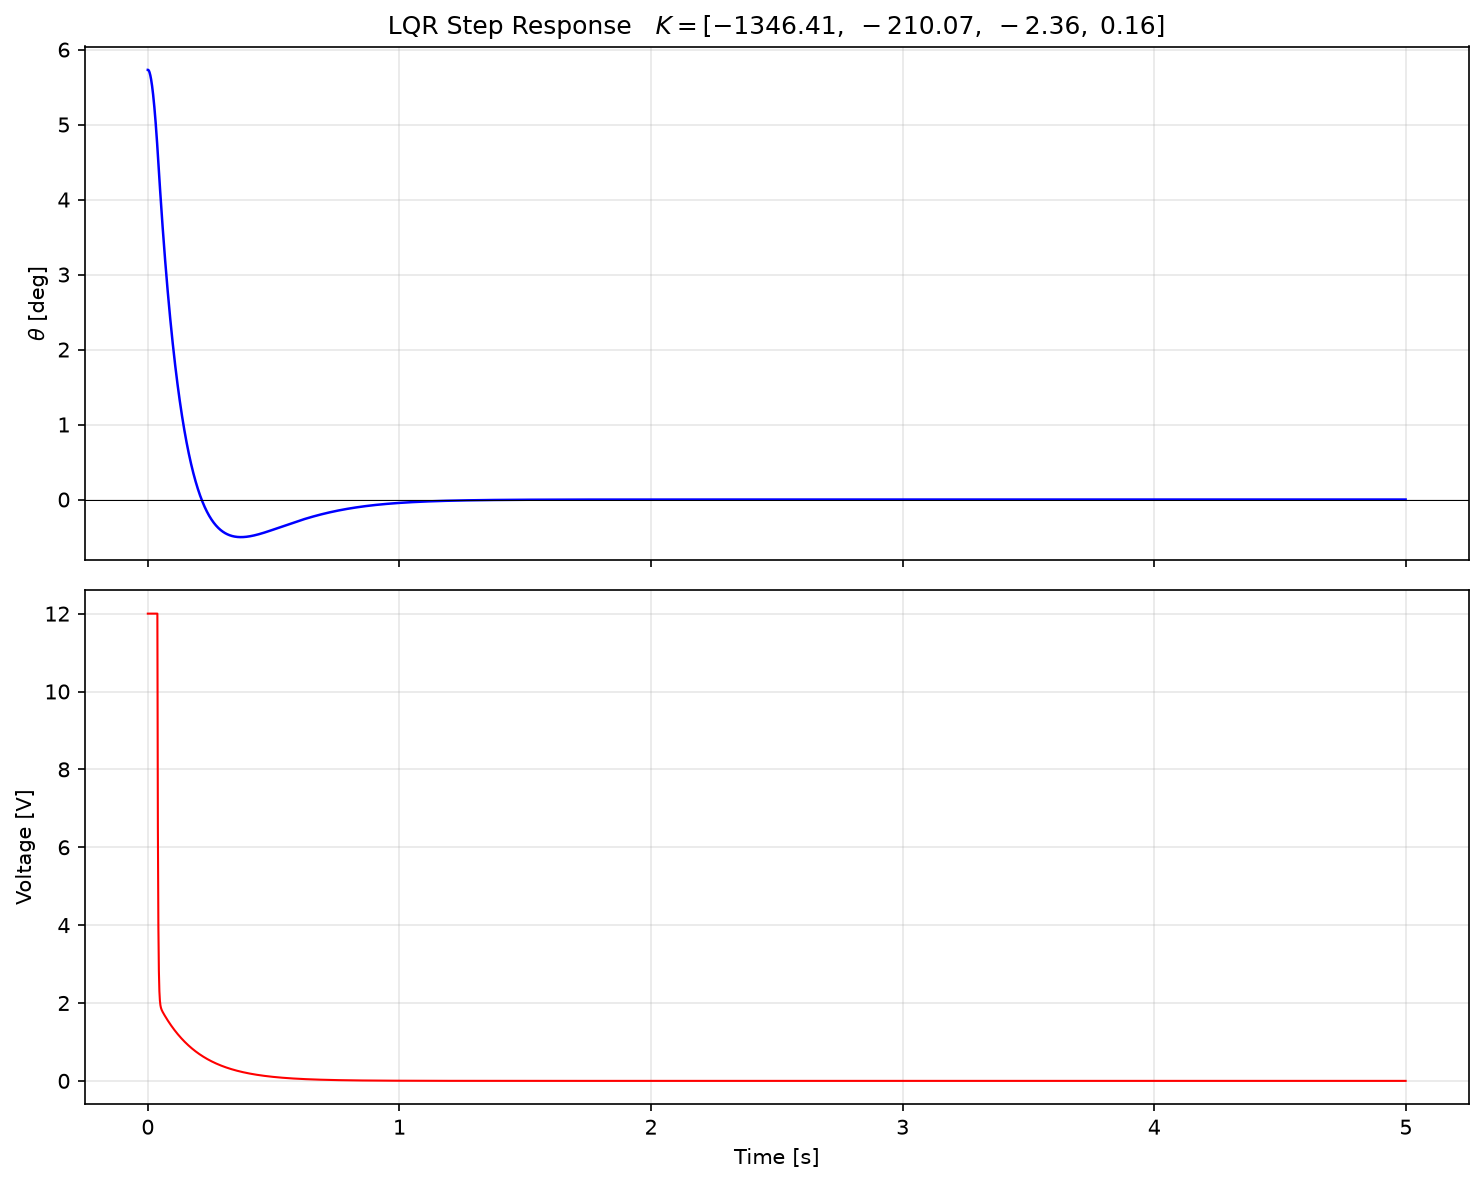
\includegraphics[width=0.85\textwidth]{results/lqr_step_response.png}
\caption{پاسخ پله کنترلر LQR با بهره‌های بهینه ($\theta_0 = 0.1$ رادیان)}
\label{fig:lqr-step}
\end{figure}

\subsubsection{بهره‌های بهینه PID}

بهره‌های PID با کمینه‌سازی شاخص عملکرد ITAE (انتگرال زمان ضربدر قدر مطلق خطا) و با استفاده از الگوریتم بهینه‌سازی نلدر--مید به‌دست آمده‌اند. شرایط شبیه‌سازی: زاویه اولیه $\theta_0 = 0.1$ رادیان، افق زمانی $T = 5$ ثانیه و گام زمانی $\Delta t = 0.001$ ثانیه.

\begin{equation}
K_p = 23.21, \qquad K_i = 0.208, \qquad K_d = 5.55
\end{equation}

مقدار بهینه شاخص ITAE برابر $2.280$ است. بهره مشتقی بزرگ‌تر از بهره تناسبی نیست، اما نقش قابل‌توجهی در میرایی نوسانات ایفا می‌کند. بهره انتگرالی کوچک ولی غیرصفر، خطای ماندگار ناشی از اغتشاش‌های ثابت را جبران می‌نماید.

شکل~\ref{fig:pid-step} پاسخ پله کنترلر PID را با این بهره‌ها نشان می‌دهد.

\begin{figure}[H]
\centering
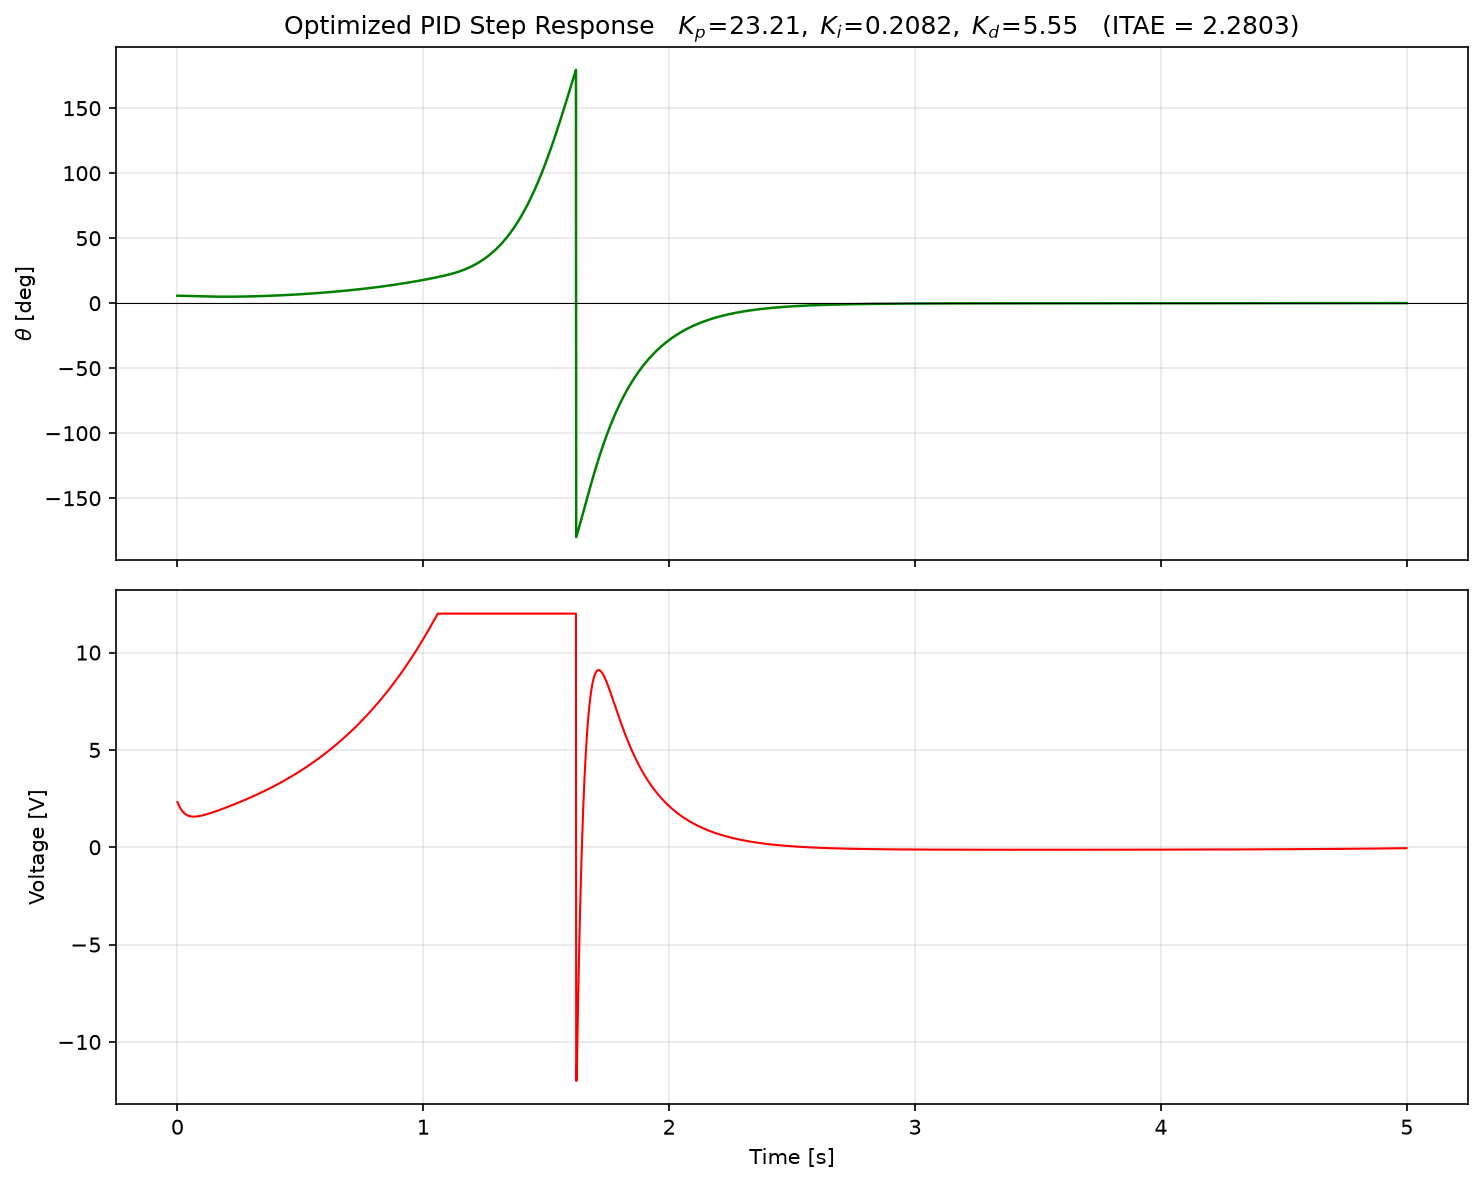
\includegraphics[width=0.85\textwidth]{results/pid_step_response.png}
\caption{پاسخ پله کنترلر PID با بهره‌های بهینه ITAE ($\theta_0 = 0.1$ رادیان)}
\label{fig:pid-step}
\end{figure}

\subsubsection{مقایسه عملکرد LQR و PID}

شکل~\ref{fig:lqr-vs-pid} مقایسه مستقیم پاسخ پله دو کنترلر را نشان می‌دهد. کنترلر LQR به دلیل استفاده از مدل کامل چهارحالته (شامل دینامیک الکتریکی) و بهینه‌سازی هم‌زمان تمام حالت‌ها، سرعت همگرایی بالاتر و نوسان کمتری نسبت به PID دارد. در مقابل، PID با ساختار ساده‌تر و تنها سه پارامتر تنظیم، پیاده‌سازی و درک شهودی آسان‌تری ارائه می‌دهد.

\begin{figure}[H]
\centering
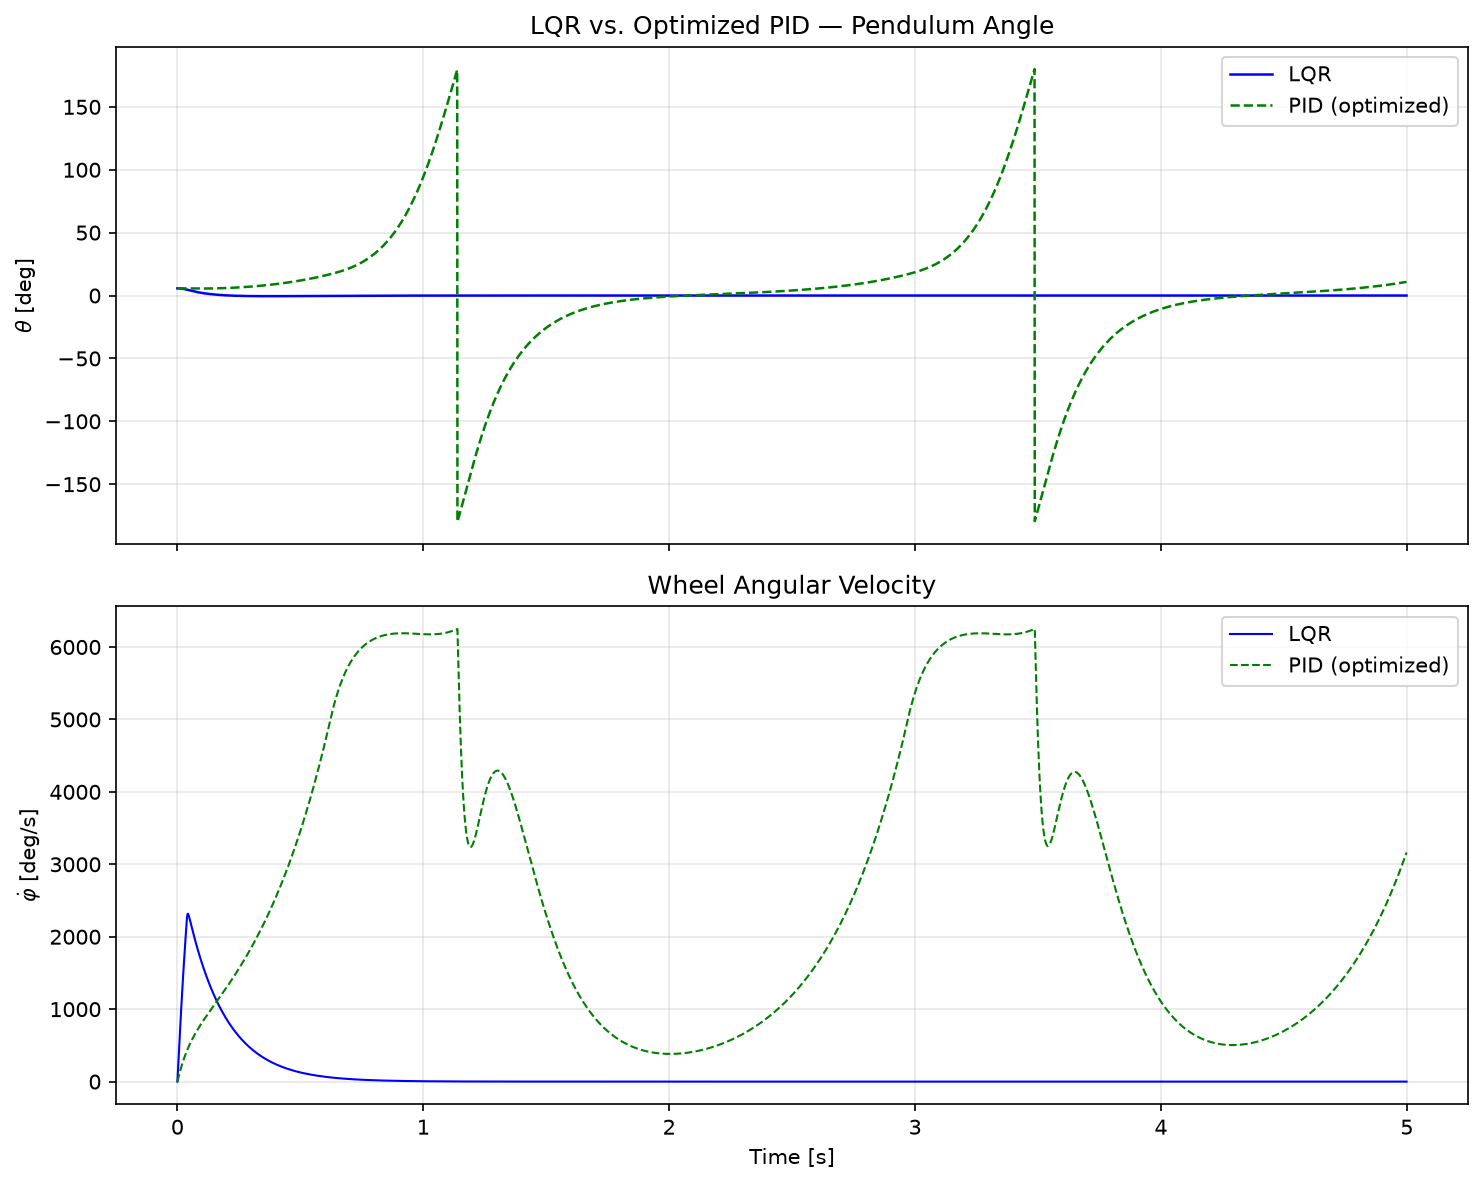
\includegraphics[width=0.85\textwidth]{results/lqr_vs_pid_comparison.png}
\caption{مقایسه پاسخ پله کنترلرهای LQR و PID ($\theta_0 = 0.1$ رادیان)}
\label{fig:lqr-vs-pid}
\end{figure}

جدول~\ref{tab:gain-summary} خلاصه‌ای از بهره‌های بهینه هر دو کنترلر را ارائه می‌دهد.

\begin{table}[H]
\centering
\caption{خلاصه بهره‌های بهینه محاسبه‌شده}
\label{tab:gain-summary}
\begin{tabular}{lll}
\toprule
\textbf{کنترلر} & \textbf{بهره‌ها} & \textbf{شاخص عملکرد} \\
\midrule
LQR & $K = [-844.46,\; -138.69,\; -2.32,\; 0.16]$ & قطب‌ها: $\approx -2374.6,\; -341.2,\; -6.12,\; -6.02$ \\
PID & $K_p = 23.21,\; K_i = 0.208,\; K_d = 5.55$ & $\text{ITAE} = 2.280$ \\
\bottomrule
\end{tabular}
\end{table}

\subsubsection{پارامترهای عددی کنترلر مد لغزشی}

پارامترهای پیش‌فرض کنترلر مد لغزشی استفاده‌شده در شبیه‌سازی‌ها به صورت زیر است:

\begin{equation}
c_1 = 10.0, \qquad c_2 = 5.0, \qquad c_3 = 1.0, \qquad K = 2.0, \qquad \eta = 0.5, \qquad \Phi = 0.05
\end{equation}

با این پارامترها، سطح لغزشی $s = 10\,\theta + 5\,\dot{\theta} + \dot{\varphi}$ تعریف می‌شود. نتایج شبیه‌سازی نشان می‌دهند که متغیر $s$ در چند صد میلی‌ثانیه نخست به لایه مرزی $|s| \le \Phi$ وارد شده و پس از آن، حرکت سیستم بر روی منیفولد لغزشی با همگرایی هموار به سمت تعادل ادامه می‌یابد. ضخامت لایه مرزی $\Phi = 0.05$ رادیان، مصالحه مناسبی بین کاهش چترینگ و حفظ دقت ردیابی ایجاد می‌کند.
\newpage
\section{الگوریتم‌های بالاآوردن}

پاندول معکوس با چرخ واکنشی یک سیستم غیرخطی و جفت‌شده است که در آن، چرخ واکنشی از طریق موتور جریان مستقیم (اتصال مستقیم، $N=1$) به پاندول کوپل شده است. هدف کنترلرهای بالاآوردن (Swing-Up) رساندن پاندول از وضعیت آویزان به وضعیت عمودی است. در این بخش، سه روش بالاآوردن پیاده‌سازی‌شده را بررسی می‌کنیم و سپس نحوه انتقال کنترل به کنترلرهای تعادلی را توضیح می‌دهیم.

برای مدل کامل دینامیک سیستم، شامل ماتریس اینرسی کوپل‌شده و معادلات مدار آرمیچر، به بخش~\ref{sec:system-math} مراجعه شود.

\subsection{مدل سیستم و مرجع انرژی}

پاندول و چرخ واکنشی یک سیستم دورانی دو‌جسمی تشکیل می‌دهند. اینرسی مؤثر چرخ، شامل اینرسی روتور موتور (در اتصال مستقیم $N=1$)، به صورت زیر تعریف می‌شود:

\begin{equation}
    I_w^{\text{eff}} = I_w + I_{\text{rotor}} \, N^2
\end{equation}

معادلات حرکت کوپل‌شده به شکل ماتریسی عبارتند از:

\begin{equation}
    \begin{bmatrix} M_{11} & M_{12} \\ M_{12} & M_{22} \end{bmatrix}
    \begin{bmatrix} \ddot{\theta} \\ \ddot{\varphi} \end{bmatrix}
    =
    \begin{bmatrix} G \sin\theta - N\,K_t\, i_a - b\,\dot\theta \\ N\,K_t\, i_a - b_w^{\text{eff}}\,\dot\varphi \end{bmatrix}
\end{equation}

که در آن جملات اینرسی به صورت زیر تعریف می‌شوند:

\begin{align}
    M_{11} &= I_p + m_w L^2 + I_w^{\text{eff}} \\
    M_{12} &= M_{22} = I_w^{\text{eff}}
\end{align}

و ضریب گرانشی، مجموع اثر وزن پاندول و چرخ را در بازوهای گشتاور مربوطه تجمع می‌دهد:

\begin{equation}
    G = \left(m_p \, \ell_{\text{com}} + m_w \, L\right) g
\end{equation}

در روابط بالا، $I_p$ اینرسی پاندول حول محور چرخش، $m_p$ و $m_w$ جرم پاندول و چرخ، $\ell_{\text{com}}$ فاصله مرکز جرم پاندول از محور، $L$ طول پاندول و $g$ شتاب گرانش است.

انرژی مکانیکی پاندول نسبت به پیکربندی سکون در وضعیت عمودی ($\theta = 0$، $\dot\theta = 0$) مرجع‌دهی می‌شود:

\begin{equation}
    E_p(\theta, \dot\theta) = \tfrac{1}{2}\, I_p\, \dot\theta^2 + G\,(\cos\theta - 1)
\end{equation}

در وضعیت عمودی، $E_p = 0$ و در پایین‌تر از عمودی، $E_p < 0$ است. هدف بالاگردان، رساندن هم‌زمان $E_p \to 0$ و $\dot\theta \to 0$ است.

\subsection{بالاآوردن مبتنی بر انرژی (روش آستروم–فوروتو)}

\subsubsection{شهود فیزیکی}

پاندول یک نوسانگر غیرخطی است. با اعمال گشتاور چرخ در فاز صحیح با نوسان پاندول، در هر نیم‌سیکل انرژی به سیستم تزریق می‌شود؛ دقیقاً مشابه عمل کودکی که با جابه‌جایی مرکز جرم خود در زمان مناسب، تاب را به ارتفاع بالاتر می‌رساند. نکته کلیدی روش آستروم–فوروتو (Åström–Furuta) این است که فقط انرژی پاندول ردیابی می‌شود، نه انرژی کل سیستم. به این ترتیب، انرژی به‌صورت غیرمفید در چرخ در حال چرخش انباشته نمی‌شود.

\subsubsection{قانون کنترل}

فرمان ولتاژ متناسب با حاصل‌ضرب کسری انرژی و سرعت چرخ است:

\begin{equation}
    V = -k_e \;\bigl(E_{\text{target}} - E_p\bigr)\; \dot\varphi
\end{equation}

که در آن $k_e > 0$ بهره انرژی (پارامتر \texttt{energy\_swing\_up\_gain}، مقدار پیش‌فرض $1.0$)، $E_{\text{target}} = 0$ ژول (انرژی سکون عمودی) و $\dot\varphi$ سرعت زاویه‌ای نسبی چرخ است. علامت منفی تضمین می‌کند که وقتی انرژی کمتر از هدف است، ولتاژ چرخ را در جهتی می‌راند که انرژی پاندول در نیم‌نوسان فعلی افزایش یابد.

\subsubsection{میرایی انرژی اضافی}

اگر پاندول از هدف انرژی فراتر رود ($E_p > 0$)، ادامه تزریق انرژی باعث چرخش پیوسته پاندول می‌شود. در این حالت، کنترلر به میرایی چرخ تغییر وضعیت می‌دهد:

\begin{equation}
    V = -\tfrac{1}{2}\, k_e\, \dot\varphi
\end{equation}

این فرمان، انرژی جنبشی چرخ را از طریق تلفات مقاومتی موتور تخلیه می‌کند.

\subsubsection{تحریک فازى}

در نزدیکی نقاط بازگشت نوسان، سرعت چرخ $\dot\varphi$ به صفر نزدیک می‌شود و سیگنال تزریق انرژی $-k_e (E_{\text{target}} - E_p) \dot\varphi$ از بین می‌رود. در نتیجه، پاندول متوقف می‌شود. برای فرار از این بن‌بست، هرگاه $|\dot\varphi| < \varphi_{\text{exc}}$ باشد (که $\varphi_{\text{exc}} = 0.5$ رادیان بر ثانیه است)، یک ولتاژ تحریک تزریق می‌شود:

\begin{equation}
    V_{\text{exc}} = \alpha\, V_{\max}\, \operatorname{sign}(\sin\theta)
\end{equation}

که در آن $\alpha = 0.3$ کسر تحریک از ولتاژ بیشینه است. جهت $\operatorname{sign}(\sin\theta)$ تضمین می‌کند که ضربه چرخ در جهتی باشد که پاندول را در نوسان بعدی به سمت بالا ببرد.

\subsubsection{کاهش تدریجی سرعت چرخ}

برای جلوگیری از شتاب‌گیری بیش از حد چرخ، ولتاژ به‌صورت خطی کاهش می‌یابد وقتی $|\dot\varphi|$ از $60\%$ سرعت بیشینه مجاز چرخ $\omega_{\max}$ فراتر رود:

\begin{equation}
    \text{scale} = \max\!\left(0,\; \frac{\omega_{\max} - |\dot\varphi|}{\omega_{\max} - 0.6\,\omega_{\max}}\right), \qquad V \leftarrow V \cdot \text{scale}
\end{equation}

این رابطه یک شیب خطی از ولتاژ کامل در $|\dot\varphi| = 0.6\,\omega_{\max}$ تا صفر در $|\dot\varphi| = \omega_{\max}$ ایجاد می‌کند.

\subsection{بالاآوردن با خطی‌سازی بازخورد جزئی}

\subsubsection{شهود فیزیکی}

روش خطی‌سازی جزئی بازخورد (Partial Feedback Linearization) رویکردی متفاوت از تزریق انرژی دارد. در این روش، به‌جای اینکه به‌صورت غیرمستقیم انرژی پاندول را افزایش دهیم، شتاب زاویه‌ای پاندول را مستقیماً فرمان می‌دهیم. ایده اصلی این است: اگر بتوانیم مشخص کنیم پاندول در هر لحظه چه شتابی باید داشته باشد، می‌توانیم از طریق معکوس‌سازی دینامیک کوپل‌شده، شتاب چرخ مورد نیاز برای تولید آن شتاب پاندول را محاسبه کنیم و سپس این شتاب چرخ را به ولتاژ موتور تبدیل نماییم.

این روش مبتنی بر مدل است؛ یعنی به دانش دقیق ماتریس اینرسی $\mathbf{M}$، ضریب گرانشی $G$ و ضرایب میرایی نیاز دارد. در مقابل روش انرژی که فقط $E_p$ را ردیابی می‌کند، خطی‌سازی بازخورد جزئی از ساختار کامل معادلات حرکت بهره می‌گیرد.

\subsubsection{شتاب مطلوب پاندول}

نخستین گام، تعریف یک شتاب مطلوب برای پاندول است. این شتاب، رفتار موردنظر پاندول را بدون توجه به چگونگی تولید آن مشخص می‌کند. برای این منظور، از یک قانون مجازی \LR{PD} (تناسبی--مشتقی) استفاده می‌کنیم. ایده این قانون ساده است: بخش تناسبی، شتابی متناسب با انحراف زاویه‌ای پاندول از وضعیت عمودی تولید می‌کند (مانند یک فنر مجازی) و بخش مشتقی، شتابی متناسب با سرعت زاویه‌ای پاندول در جهت مخالف حرکت اعمال می‌نماید (مانند یک میراگر مجازی). بدون بخش مشتقی، پاندول حول نقطه هدف نوسان بی‌پایان انجام می‌داد؛ این بخش، انرژی جنبشی مجازی را در هر نیم‌سیکل تخلیه می‌کند و همگرایی مجانبی را تضمین می‌نماید.

قانون مجازی \LR{PD} به صورت زیر تعریف می‌شود:

\begin{equation}
    \ddot\theta_{\text{des}} = -k_p \sin\theta - k_d\, \dot\theta
\end{equation}

در این رابطه، $k_p^{\text{PFL}}$ بهره تناسبی و $k_d^{\text{PFL}}$ بهره مشتقی قانون مجازی \LR{PD} هستند.

\paragraph{نقش فیزیکی $k_p^{\text{PFL}}$ (بهره تناسبی).}
جمله $-k_p \sin\theta$ یک شتاب بازگرداننده وابسته به موقعیت ایجاد می‌کند؛ معادل یک فنر مجازی غیرخطی که پاندول را به سمت $\theta = 0$ می‌کشاند. استفاده از $\sin\theta$ به‌جای $\theta$ ضروری است، زیرا این کنترلر باید در تمام زوایا (نه فقط نزدیکی عمودی) کار کند. در نزدیکی افقی، $|\sin\theta| \approx 1$ و شتاب بازگرداننده بیشینه است؛ در نزدیکی عمودی، $\sin\theta \to 0$ و شتاب به‌صورت طبیعی کاهش می‌یابد. هرچه $k_p^{\text{PFL}}$ بزرگ‌تر باشد، شتاب بازگرداننده قوی‌تر و همگرایی سریع‌تر است؛ اما مقادیر بیش از حد بزرگ، فرمان‌های شتاب چرخ بسیار بزرگی تولید می‌کنند که ممکن است از محدودیت‌های ولتاژ و سرعت چرخ فراتر روند.

\paragraph{نقش فیزیکی $k_d^{\text{PFL}}$ (بهره مشتقی).}
جمله $-k_d \dot\theta$ میرایی سرعتی فراهم می‌کند و نقش یک دمپر (میراگر) مجازی را ایفا می‌نماید. بدون این جمله، قانون مجازی به $\ddot\theta_{\text{des}} = -k_p \sin\theta$ تقلیل می‌یابد که یک نوسانگر بدون اتلاف است و پاندول به‌جای همگرایی به $\theta = 0$، در اطراف آن نوسان پایدار انجام می‌دهد. جمله میرایی، انرژی جنبشی مجازی سیستم را در هر نیم‌سیکل تخلیه می‌کند و نوسانات اطراف نقطه هدف را به‌تدریج از بین می‌برد. به بیان دیگر، $k_d^{\text{PFL}}$ مشخص می‌کند که پاندول با چه سرعتی از نوسان باز می‌ایستد و به حالت سکون در وضعیت عمودی می‌رسد.

\paragraph{تنظیم بهره‌ها.}
در نزدیکی وضعیت عمودی ($\sin\theta \approx \theta$)، قانون مجازی به معادله خطی مرتبه دوم زیر تبدیل می‌شود:

\begin{equation}
    \ddot\theta + k_d^{\text{PFL}}\, \dot\theta + k_p^{\text{PFL}}\, \theta = 0
\end{equation}

این معادله یک نوسانگر میرای مرتبه دوم است که دو پارامتر مشخصه دارد:

\begin{equation}
    \omega_n = \sqrt{k_p^{\text{PFL}}}, \qquad \zeta = \frac{k_d^{\text{PFL}}}{2\sqrt{k_p^{\text{PFL}}}}
\end{equation}

که در آن‌ها $\omega_n$ فرکانس طبیعی (تعیین‌کننده سرعت همگرایی) و $\zeta$ نسبت میرایی (تعیین‌کننده مقدار نوسان) است. بر این اساس، تنظیم بهره‌ها در دو گام انجام می‌شود:

\begin{enumerate}
    \item \textbf{انتخاب $\omega_n$:} فرکانس طبیعی مجازی باید به‌اندازه کافی بزرگ باشد که همگرایی در چند ثانیه حاصل شود، اما از پهنای باند عملی موتور فراتر نرود. محدوده مناسب $\omega_n \in [2,\; 3]$ \LR{rad/s} است. سپس $k_p^{\text{PFL}} = \omega_n^2$ قرار می‌دهیم.
    \item \textbf{انتخاب $\zeta$:} مقدار $\zeta = 1$ (میرایی بحرانی) سریع‌ترین همگرایی بدون نوسان را فراهم می‌کند. مقادیر $\zeta < 1$ پاسخ نوسانی میرا و $\zeta > 1$ همگرایی کندتر بدون نوسان تولید می‌کنند. سپس $k_d^{\text{PFL}} = 2\zeta\,\omega_n$ قرار می‌دهیم.
\end{enumerate}

\paragraph{قید شتاب و بررسی عددی.}
بهره‌های انتخابی باید در محدودیت فیزیکی موتور قابل تحقق باشند. حداکثر شتاب پاندول که موتور می‌تواند تولید کند، از روابط زیر به دست می‌آید:

\begin{equation}
    i_{\max} = \frac{V_{\max}}{R_a} = \frac{12}{1.2} = 10\;\text{A}, \qquad
    \tau_{\max} = K_t \, i_{\max} = 0.876\;\text{N·m}
\end{equation}

\begin{equation}
    \ddot\varphi_{\max} = \frac{\tau_{\max}}{I_{w,\text{eff}}} \approx 1230\;\text{rad/s}^2, \qquad
    \ddot\theta_{\max} \approx \ddot\varphi_{\max} \cdot \frac{M_{12}}{M_{11}} \approx 16\;\text{rad/s}^2
\end{equation}

در بدترین حالت ($\theta = \pi/2$ و $\dot\theta \approx 2$ \LR{rad/s})، شتاب مطلوب برابر $k_p^{\text{PFL}} + 2\,k_d^{\text{PFL}}$ است و باید کمتر از $16$ \LR{rad/s²} باقی بماند.

با انتخاب $\zeta = 1$ و $\omega_n = 2.2$ \LR{rad/s}:

\begin{equation}
    k_p^{\text{PFL}} = \omega_n^2 = 4.84 \approx 5.0, \qquad
    k_d^{\text{PFL}} = 2\zeta\,\omega_n = 4.4 \approx 4.5
\end{equation}

بررسی قید: $5.0 + 2 \times 4.5 = 14.0 < 16$ ✓. این مقادیر، میرایی بحرانی با زمان همگرایی حدود $2$ ثانیه فراهم می‌کنند و در محدوده عملی موتور قرار دارند. مقادیر پیش‌فرض پیاده‌سازی ($k_p^{\text{PFL}} = 5.0$، $k_d^{\text{PFL}} = 2.0$) متناظر با $\zeta \approx 0.45$ هستند و پاسخ نوسانی میرا تولید می‌کنند.

این دو جمله در کنار هم، یک میدان برداری پایدار به سمت $\theta = 0$ شکل می‌دهند. به بیان دیگر، اگر پاندول بتواند دقیقاً از $\ddot\theta_{\text{des}}$ پیروی کند، به‌صورت مجانبی به وضعیت عمودی همگرا می‌شود.

\subsubsection{معکوس‌سازی دینامیک}

اکنون پرسش اصلی این است: چه شتاب چرخی $\ddot\varphi$ لازم است تا پاندول شتاب $\ddot\theta_{\text{des}}$ را تجربه کند؟ برای پاسخ، از سطر اول معادلات کوپل‌شده حرکت شروع می‌کنیم:

\begin{equation}
    M_{11}\,\ddot\theta + M_{12}\,\ddot\varphi = G\sin\theta - N\,K_t\, i_a - b\,\dot\theta
\end{equation}

در این رابطه، سمت چپ شامل جملات اینرسی (شتاب‌های پاندول و چرخ) و سمت راست شامل نیروهای فعال (گرانش، گشتاور موتور و میرایی) است. حال $\ddot\theta = \ddot\theta_{\text{des}}$ را جایگذاری می‌کنیم و معادله را برای $\ddot\varphi$ حل می‌نماییم:

\begin{equation}
    M_{12}\,\ddot\varphi = G\sin\theta - N\,K_t\, i_a - b\,\dot\theta - M_{11}\,\ddot\theta_{\text{des}}
\end{equation}

و در نتیجه:

\begin{equation}
    \boxed{\ddot\varphi_{\text{req}} = \frac{G\sin\theta - N\,K_t\, i_a - b\,\dot\theta - M_{11}\,\ddot\theta_{\text{des}}}{M_{12}}}
\end{equation}

این رابطه، هسته خطی‌سازی بازخورد جزئی است. با محاسبه $\ddot\varphi_{\text{req}}$، عملاً جملات غیرخطی گرانش ($G\sin\theta$) و میرایی ($-b\dot\theta$) و اثر جریان لحظه‌ای آرمیچر ($-N K_t i_a$) را جبران می‌کنیم و رفتار پاندول را با رفتار خطی موردنظر ($\ddot\theta_{\text{des}}$) جایگزین می‌نماییم.

واژه «جزئی» در نام این روش به این دلیل است که فقط کانال پاندول خطی می‌شود. دینامیک داخلی چرخ (که از سطر دوم معادلات به دست می‌آید) همچنان غیرخطی باقی می‌ماند و می‌تواند مقادیر بزرگ $\ddot\varphi_{\text{req}}$ تولید کند. به همین دلیل، لایه‌های حفاظتی سرعت چرخ ضروری هستند.

نقش درایه غیرقطری $M_{12}$ در این رابطه محوری است. این کمیت، جفت‌شدگی سینتیکی بین پاندول و چرخ را بیان می‌کند و تنها مکانیزمی است که از طریق آن شتاب چرخ بر شتاب پاندول اثر می‌گذارد. با مقادیر پیش‌فرض، $M_{12}/M_{11} \approx 0.013$ است؛ بنابراین برای تولید یک واحد شتاب پاندول، به حدود $77$ واحد شتاب چرخ نیاز است. این نسبت، نیاز به سرعت‌های بالای چرخ در روش‌های بالاآوردن را توضیح می‌دهد.

\subsubsection{نگاشت گشتاور و ولتاژ}

پس از محاسبه $\ddot\varphi_{\text{req}}$، باید مشخص کنیم چه گشتاور موتوری این شتاب چرخ را هم‌زمان با حفظ $\ddot\theta_{\text{des}}$ تولید می‌کند. از سطر دوم معادلات کوپل‌شده استفاده می‌کنیم:

\begin{equation}
    M_{12}\,\ddot\theta + M_{22}\,\ddot\varphi = N\,K_t\, i_a - b_{w,\text{eff}}\,\dot\varphi
\end{equation}

با جایگذاری $\ddot\theta = \ddot\theta_{\text{des}}$ و $\ddot\varphi = \ddot\varphi_{\text{req}}$ و صرف‌نظر از جمله میرایی چرخ $b_{w,\text{eff}}\dot\varphi$ (که در مقایسه با جملات اینرسی کوچک است)، گشتاور موتور به صورت زیر به دست می‌آید:

\begin{equation}
    N\,K_t\, i_a = M_{12}\,\ddot\theta_{\text{des}} + M_{22}\,\ddot\varphi_{\text{req}}
\end{equation}

از آنجا که $\tau_m = K_t\, i_a$، گشتاور موتور مورد نیاز برابر است با:

\begin{equation}
    \boxed{\tau_m = \frac{M_{12}\,\ddot\theta_{\text{des}} + M_{22}\,\ddot\varphi_{\text{req}}}{N}}
\end{equation}

در اتصال مستقیم ($N = 1$)، این رابطه ساده‌تر می‌شود: $\tau_m = M_{12}\,\ddot\theta_{\text{des}} + M_{22}\,\ddot\varphi_{\text{req}}$.

گام نهایی، تبدیل گشتاور به ولتاژ است. مدار آرمیچر موتور DC از رابطه زیر پیروی می‌کند:

\begin{equation}
    V = R_a\, i_a + L_a \frac{di_a}{dt} + K_e\, N\, \dot\varphi
\end{equation}

ثابت زمانی الکتریکی $\tau_e = L_a / R_a \approx 0.42$ میلی‌ثانیه است، در حالی که مقیاس زمانی مکانیکی سیستم حدود $155$ میلی‌ثانیه (معادل $1/\omega_n$) است. این اختلاف دو مرتبه بزرگی، فرض شبه‌ایستای الکتریکی را توجیه می‌کند: $L_a\, di_a/dt \approx 0$. با این ساده‌سازی و جایگذاری $i_a = \tau_m / K_t$:

\begin{equation}
    \boxed{V = R_a \frac{\tau_m}{K_t} + K_e\, N\, \dot\varphi}
\end{equation}

هر یک از دو جمله این رابطه نقش فیزیکی مشخصی دارد:

\begin{itemize}
    \item \textbf{جمله اول} ($R_a\, \tau_m / K_t$): ولتاژ مقاومتی لازم برای ایجاد جریان آرمیچری که گشتاور $\tau_m$ را تولید کند. این جمله، بخش اصلی فرمان ولتاژ است.
    \item \textbf{جمله دوم} ($K_e\, N\, \dot\varphi$): جبران نیروی ضد محرکه الکتریکی (Back-EMF). چرخ در حال چرخش، ولتاژی متناسب با سرعت خود تولید می‌کند که با ولتاژ اعمالی مقابله می‌نماید. بدون این جبران، در سرعت‌های بالای چرخ، ولتاژ مؤثر آرمیچر به‌شدت کاهش می‌یابد و موتور قادر به تولید گشتاور مورد نیاز نخواهد بود.
\end{itemize}

\subsubsection{اشباع آگاه از انرژی}

اگر انرژی پاندول به هدف عمودی رسیده یا از آن فراتر رفته باشد ($E_p > 0$)، ادامه شتاب‌دهی باعث فراجهش از وضعیت عمودی می‌شود. در این حالت، کنترلر به حالت ترمز Back-EMF تغییر وضعیت می‌دهد:

\begin{equation}
    V = -K_e\, N\, \dot\varphi
\end{equation}

این فرمان معادل اتصال کوتاه الکتریکی موتور است: ولتاژ خارجی صفر قرار می‌گیرد و Back-EMF تولیدشده توسط چرخ، جریانی از طریق مقاومت آرمیچر هدایت می‌کند. این جریان، گشتاور ترمزی مخالف جهت چرخش ایجاد می‌کند و انرژی جنبشی چرخ را به حرارت در $R_a$ تبدیل می‌سازد. در نتیجه، سرعت چرخ کاهش می‌یابد و از شتاب‌دهی بیشتر پاندول جلوگیری می‌شود.

\subsection{بالاآوردن ضربه‌ای در سرعت صفر}

\subsubsection{شهود فیزیکی}

این روش مستقیم‌ترین راهبرد است: صبر می‌کنیم تا پاندول به نقطه بازگشت نوسان برسد (جایی که لحظه‌ای متوقف می‌شود)، سپس یک ضربه گشتاور شدید به چرخ وارد می‌کنیم. بر اساس پایستگی تکانه زاویه‌ای، پاندول یک ضربه زاویه‌ای مساوی و در جهت مخالف دریافت می‌کند و با انرژی بیشتری به مسیر خود بازمی‌گردد. تکرار این فرایند در هر نقطه بازگشت، دامنه نوسان را به‌تدریج افزایش می‌دهد.

\subsubsection{تشخیص عبور از صفر}

پاندول در نقطه بازگشت نوسان قرار دارد وقتی سرعت زاویه‌ای آن تغییر علامت دهد:

\begin{equation}
    (\dot\theta_{\text{prev}} > 0 \;\wedge\; \dot\theta \leq 0) \quad \lor \quad (\dot\theta_{\text{prev}} < 0 \;\wedge\; \dot\theta \geq 0)
\end{equation}

ضربه فقط در صورتی فعال می‌شود که $|\theta| > \theta_{\min} = 0.05$ رادیان باشد (برای جلوگیری از تحریک کاذب در نزدیکی تعادل عمودی) و انرژی پاندول هنوز کمتر از هدف باشد ($E_p < 0$).

\subsubsection{قانون ضربه}

در نقطه بازگشت شناسایی‌شده، یک ولتاژ ثابت به مدت $\Delta t_{\text{imp}}$ اعمال می‌شود:

\begin{equation}
    V = \operatorname{sign}(\theta) \cdot V_{\max}, \qquad t \in [0,\; \Delta t_{\text{imp}}]
\end{equation}

تعداد گام‌های انتگرال‌گیری $\lceil \Delta t_{\text{imp}} / h \rceil$ است که $h$ گام زمانی فیزیک است. قرارداد علامت $\operatorname{sign}(\theta)$ تضمین می‌کند که گشتاور واکنشی چرخ، پاندول را در نوسان برگشتی به سمت عمودی هل می‌دهد. وقتی $\theta > 0$ (پاندول به راست کج شده)، ولتاژ مثبت چرخ را در جهت مثبت شتاب می‌دهد و واکنش آن پاندول را به سمت عمودی بازمی‌گرداند.

\subsubsection{قطع ایمنی}

اگر در حین یک ضربه فعال، سرعت چرخ از $0.9\,\omega_{\max}$ فراتر رود، ضربه فوراً قطع شده و ولتاژ به صفر بازمی‌گردد. این مکانیزم از سرعت بیش از حد چرخ ناشی از ضربات متوالی جلوگیری می‌کند.

\subsection{تحلیل مقایسه‌ای و انتخاب روش بهینه}

پس از معرفی سه روش بالاآوردن، این پرسش مطرح می‌شود که کدام یک برای سیستم مورد بررسی مناسب‌تر است. پاسخ به این پرسش را می‌توان از دل خود دینامیک سیستم و با محاسبه نسبت‌های بی‌بعد مشخصه استخراج کرد. در این subsection، ابتدا نرخ انتقال انرژی از چرخ به پاندول را از معادلات کوپل‌شده مشتق می‌کنیم، سپس با ارزیابی عددی پارامترها، هر سه روش را در برابر محدودیت‌های فیزیکی سیستم می‌سنجیم.

\subsubsection{نسبت‌های مشخصه سیستم}

پیش از تحلیل، مقادیر عددی چند نسبت کلیدی را با پارامترهای پیش‌فرض جدول~\ref{tab:computed-values} محاسبه می‌کنیم:

\begin{table}[H]
\centering
\caption{نسبت‌های مشخصه تعیین‌کننده انتخاب الگوریتم بالاآوردن}
\label{tab:ratios}
\begin{tabular}{lccl}
\toprule
\textbf{کمیت} & \textbf{مقدار} & \textbf{مقیاس مکانیکی} & \textbf{نتیجه} \\
\midrule
ثابت زمانی الکتریکی $\tau_e = L_a/R_a$ & $0.42$ \LR{ms} & $T/2 \approx 490$ \LR{ms} & $\tau_e \ll T$ \\
نسبت کوپل $M_{12}/M_{11}$ & $0.013$ & --- & کوپل ضعیف \\
گشتاور بیشینه موتور $K_t V_{\max}/R_a$ & $0.876$ \LR{N·m} & $G = 2.21$ \LR{N·m} & $\tau_{\max} \approx 0.4\,G$ \\
تکانه زاویه‌ای چرخ در $\omega_{\max}$ & $0.036$ \LR{N·m·s} & $\mathcal{L}_p \approx 0.18$ \LR{N·m·s} & $\approx 20\%$ \\
\bottomrule
\end{tabular}
\end{table}

این اعداد چهار نتیجه فوری دارند:

\begin{enumerate}
    \item ثابت زمانی الکتریکی ($0.42$ میلی‌ثانیه) در مقایسه با نیم‌دوره نوسان پاندول ($490$ میلی‌ثانیه) سه مرتبه بزرگی کوچک‌تر است. بنابراین، جریان آرمیچر تقریباً بدون تأخیر از ولتاژ پیروی می‌کند و فرمان‌های ولتاژ بی‌درنگ به گشتاور تبدیل می‌شوند.
    \item نسبت کوپل $M_{12}/M_{11} \approx 0.013$ نشان می‌دهد که اینرسی چرخ تنها $1.3\%$ اینرسی کل سیستم است. برای تولید یک واحد شتاب پاندول، به حدود $77$ واحد شتاب چرخ نیاز است. این کوپل ضعیف، نیاز به چندین نوسان برای انباشت انرژی را اجتناب‌ناپذیر می‌سازد.
    \item گشتاور بیشینه موتور ($0.876$ \LR{N·m}) تنها $40\%$ گشتاور گرانشی ($2.21$ \LR{N·m}) است. موتور نمی‌تواند پاندول را به‌صورت استاتیکی در وضعیت افقی نگه دارد و صرفاً از طریق دینامیک ضربه‌ای و نوسانی قادر به بالاآوردن است.
    \item تکانه زاویه‌ای چرخ در سرعت بیشینه ($50$ \LR{rad/s}) حدود $20\%$ تکانه زاویه‌ای پاندول در اواسط نوسان است. این نسبت، تعداد نوسان‌های مورد نیاز برای بالاآوردن کامل را تعیین می‌کند.
\end{enumerate}

\subsubsection{مشتق نرخ انتقال انرژی}

برای درک مکانیزم انتقال انرژی از چرخ به پاندول، مشتق زمانی انرژی پاندول $E_p = \tfrac{1}{2}I_p\dot\theta^2 + G(\cos\theta - 1)$ را محاسبه می‌کنیم:

\begin{equation}
    \frac{dE_p}{dt} = I_p\,\dot\theta\,\ddot\theta - G\sin\theta\,\dot\theta
    = \dot\theta\!\left(I_p\,\ddot\theta - G\sin\theta\right)
\end{equation}

از سطر اول معادلات کوپل‌شده، شتاب پاندول برابر است با:

\begin{equation}
    \ddot\theta = \frac{G\sin\theta - NK_t\, i_a - b\,\dot\theta - M_{12}\,\ddot\varphi}{M_{11}}
\end{equation}

با جایگذاری در رابطه انرژی و ساده‌سازی، بخش قابل‌کنترل نرخ تغییرات انرژی (جملاتی که ولتاژ $V$ بر آن‌ها اثر می‌گذارد) به صورت زیر به دست می‌آید:

\begin{equation}
    \boxed{\frac{dE_p}{dt}\bigg|_{\text{ctrl}}
    = -\frac{I_p}{M_{11}}\,\dot\theta\!\left(NK_t\, i_a + M_{12}\,\ddot\varphi\right)}
\end{equation}

این رابطه، هسته فیزیکی انتخاب الگوریتم بهینه است. دو نتیجه مستقیم از آن استخراج می‌شود:

\begin{itemize}
    \item \textbf{شرط تزریق انرژی:} برای اینکه $dE_p/dt > 0$ باشد، عبارت داخل پرانتز باید خلاف علامت $\dot\theta$ باشد. به بیان دیگر، وقتی پاندول در جهت مثبت حرکت می‌کند ($\dot\theta > 0$)، گشتاور موتور و شتاب چرخ باید در جهتی باشند که انرژی به پاندول تزریق شود.
    \item \textbf{نقش کوپل ضعیف:} ضریب $I_p/M_{11} \approx 0.56$ نشان می‌دهد که تنها حدود $56\%$ انرژی جنبشی پاندول مستقیماً از طریق اینرسی پاندول قابل کنترل است. باقی‌مانده از طریق جملات کوپل $M_{12}$ منتقل می‌شود که ضریب کوچک $0.013$ دارد.
\end{itemize}

با توجه به اینکه $\tau_e \ll \Delta t$، جریان آرمیچر به‌صورت شبه‌ایستا از رابطه $i_a \approx (V - K_e N\dot\varphi)/R_a$ پیروی می‌کند. بنابراین، فرمان ولتاژ $V$ تقریباً بی‌درنگ به گشتاور موتور و در نتیجه به نرخ انتقال انرژی تبدیل می‌شود.

\subsubsection{ارزیابی روش انرژی (آستروم–فوروتو)}

قانون کنترل $V = -k_e(E_{\text{target}} - E_p)\dot\varphi$ را در رابطه نرخ انرژی جایگذاری می‌کنیم. شتاب چرخ $\ddot\varphi$ متناسب با گشتاور موتور و در نتیجه متناسب با $V$ است. نرخ انتقال انرژی حاصل:

\begin{equation}
    \frac{dE_p}{dt}\bigg|_{\text{energy}} \propto (E_{\text{target}} - E_p)\,\dot\varphi\,\dot\theta
\end{equation}

این عبارت در طول یک دوره کامل نوسان، به‌طور متوسط مثبت است. دلیل این امر، همبستگی فاز بین $\dot\varphi$ و $\dot\theta$ از طریق کوپل $M_{12}$ است. ویژگی‌های کلیدی این روش عبارتند از:

\begin{itemize}
    \item \textbf{زمان‌بندی خودکار بهره:} کسری انرژی $(E_{\text{target}} - E_p)$ به‌عنوان یک بهره متغیر عمل می‌کند. در ابتدای بالاآوردن (انرژی بسیار منفی)، پمپاژ قوی انجام می‌شود؛ در نزدیکی عمودی (انرژی نزدیک صفر)، پمپاژ به‌صورت طبیعی ملایم می‌گردد.
    \item \textbf{عدم نیاز به معکوس‌سازی مدل:} این روش از ساختار کامل ماتریس اینرسی استفاده نمی‌کند و تنها به علامت $\dot\varphi$ و مقدار عددی $E_p$ نیاز دارد. در نتیجه، به خطاهای پارامتری در $M_{12}$ و $G$ حساس نیست.
    \item \textbf{پایداری لیاپانوف:} تابع کاندید $V_p = \tfrac{1}{2}(E_p - E_{\text{target}})^2$ دارای مشتق $\dot{V}_p \leq 0$ است که همگرایی مجانبی انرژی به هدف را تضمین می‌کند.
\end{itemize}

\subsubsection{ارزیابی روش خطی‌سازی بازخورد جزئی}

روش \LR{PFL} شتاب چرخ مورد نیاز را از رابطه $\ddot\varphi_{\text{req}} = (G\sin\theta - M_{11}\ddot\theta_{\text{des}})/M_{12}$ محاسبه می‌کند. با $M_{12} = 0.0007125$ \LR{kg·m²}، تقسیم بر این مقدار کوچک، حساسیت بالایی به خطاهای پارامتری ایجاد می‌کند:

\begin{equation}
    \frac{\partial \ddot\varphi_{\text{req}}}{\partial M_{12}} = -\frac{G\sin\theta - M_{11}\ddot\theta_{\text{des}}}{M_{12}^2}
\end{equation}

یک خطای $10\%$ در $M_{12}$، خطای $10\%$ در $\ddot\varphi_{\text{req}}$ و در نتیجه خطای معادل در ولتاژ فرمان تولید می‌کند. علاوه بر این، فرض شبه‌ایستای الکتریکی ($L_a\, di_a/dt \approx 0$) در این روش نقش محوری دارد. نسبت $\tau_e / \Delta t = 0.42$ نشان می‌دهد که این فرض در فرکانس $1$ کیلوهرتز قابل‌قبول است، اما در گذراهای سریع (نزدیک اشباع ولتاژ)، تأخیر فاز کوچکی ایجاد می‌شود.

مزیت اصلی \LR{PFL}، همگرایی سریع‌تر در هر نوسان است. این روش به‌جای پمپاژ تدریجی انرژی، مستقیماً شتاب پاندول را فرمان می‌دهد و در صورت دقت مدل، مسیر بهینه‌تری را طی می‌کند.

\subsubsection{ارزیابی روش ضربه‌ای}

روش ضربه‌ای ولتاژ کامل را در لحظه عبور سرعت پاندول از صفر اعمال می‌کند. در این لحظه، $\dot\theta \approx 0$ برقرار است. با مراجعه به رابطه نرخ انتقال انرژی:

\begin{equation}
    \frac{dE_p}{dt}\bigg|_{\text{ctrl}} = -\frac{I_p}{M_{11}}\,\dot\theta\!\left(NK_t\, i_a + M_{12}\,\ddot\varphi\right) \approx 0
\end{equation}

در نقطه بازگشت، $\dot\theta \approx 0$ و بنابراین نرخ انتقال انرژی به پاندول تقریباً صفر است. ضربه ولتاژ در این لحظه، عمدتاً انرژی جنبشی چرخ را افزایش می‌دهد و تنها در نوسان بعدی (وقتی $\dot\theta \neq 0$ می‌شود) بخشی از این انرژی به پاندول منتقل می‌گردد. این تأخیر ذاتی در انتقال انرژی، روش ضربه‌ای را از نظر بهره‌وری در رتبه آخر قرار می‌دهد.

\subsubsection{نتیجه‌گیری و توصیه}

جدول~\ref{tab:comparison} مقایسه سه روش را بر اساس معیارهای استخراج‌شده از دینامیک سیستم خلاصه می‌کند.

\begin{table}[H]
\centering
\caption{مقایسه روش‌های بالاآوردن بر اساس دینامیک سیستم}
\label{tab:comparison}
\begin{tabular}{lccc}
\toprule
\textbf{معیار} & \textbf{انرژی} & \textbf{\LR{PFL}} & \textbf{ضربه‌ای} \\
\midrule
تعداد نوسان تا عمودی & متوسط & کم & زیاد \\
حساسیت به خطای پارامتری & کم & زیاد & کم \\
بهره‌وری انتقال انرژی & بالا & بالا & پایین \\
نیاز به دقت مدل & ندارد & دارد & ندارد \\
پیچیدگی پیاده‌سازی & کم & متوسط & کم \\
\bottomrule
\end{tabular}
\end{table}

با توجه به کوپل ضعیف ($M_{12}/M_{11} \approx 0.013$)، گشتاور محدود موتور ($\tau_{\max} \approx 0.4\,G$) و ضرورت انباشت انرژی در چندین نوسان، \textbf{روش انرژی (آستروم–فوروتو) مناسب‌ترین انتخاب برای این سیستم} است. دلایل این انتخاب مستقیماً از دینامیک سیستم پیروی می‌کنند:

\begin{enumerate}
    \item کوپل ضعیف، بالاآوردن تک‌نوسانه را غیرممکن می‌سازد. روش انرژی به‌طور طبیعی انرژی را در چندین نوسان انباشته می‌کند.
    \item محدودیت گشتاور موتور، اشباع ولتاژ را در هر نوسان اجتناب‌ناپذیر می‌سازد. زمان‌بندی خودکار بهره در روش انرژی، از اشباع بی‌مورد جلوگیری می‌کند.
    \item حساسیت پایین به خطاهای پارامتری، این روش را در برابر عدم‌قطعیت مدل (که در سیستم‌های واقعی اجتناب‌ناپذیر است) مقاوم می‌سازد.
\end{enumerate}

در صورت نیاز به همگرایی سریع‌تر، یک رویکرد ترکیبی قابل‌تصور است: استفاده از روش انرژی برای $|\theta| > 0.5$ رادیان و سوئیچ به \LR{PFL} در ناحیه $0.3 < |\theta| < 0.5$ رادیان. با این حال، برای پارامترهای پیش‌فرض این سیستم، روش انرژی به‌تنهایی عملکرد کافی و قابل‌اطمینان ارائه می‌دهد.

\subsection{انتقال به کنترل تعادلی}

کنترلرهای بالاآوردن فقط در فاصله زیاد از وضعیت عمودی مؤثر هستند. در نزدیکی نقطه تعادل، یک کنترلر تعادلی پایدارساز کنترل را در دست می‌گیرد. شرط انتقال، قرار گرفتن هم‌زمان زاویه و سرعت در آستانه‌های مشخص است:

\begin{equation}
    |\theta| < \theta_{\text{up}} \quad \wedge \quad |\dot\theta| < \dot\theta_{\text{up}}
\end{equation}

که مقادیر پیش‌فرض $\theta_{\text{up}} = 0.3$ رادیان و $\dot\theta_{\text{up}} = 1.0$ رادیان بر ثانیه هستند.

پس از برقراری شرط انتقال، بسته به حالت انتخابی، کنترلر LQR یا PID فعال می‌شود. برای فرمول‌بندی کامل این کنترل‌کننده‌ها، به بخش~\ref{sec:controllers} مراجعه شود.

\subsection{قیدهای ایمنی سراسری}

تمام روش‌های بالاآوردن در یک طرح حفاظتی چندلایه پیچیده شده‌اند که مستقل از الگوریتم انتخابی عمل می‌کند. جدول~\ref{tab:safety} این لایه‌ها را خلاصه می‌کند.

\begin{table}[H]
\centering
\caption{لایه‌های حفاظتی سرعت چرخ و ولتاژ}
\label{tab:safety}
\begin{tabular}{lll}
\toprule
\textbf{لایه} & \textbf{شرط} & \textbf{اثر} \\
\midrule
محافظ سخت سرعت & $|\dot\varphi| > 1.5\,\omega_{\max}$ & $V = 0$ (قطع فوری) \\
فرمانده سرعت & $|\dot\varphi| \geq \omega_{\max}$ & $V = 0$ \\
کاهش باند بالا & $|\dot\varphi| > 0.6\,\omega_{\max}$ & $V \leftarrow V \cdot \dfrac{\omega_{\max} - |\dot\varphi|}{0.4\,\omega_{\max}}$ \\
اشباع ولتاژ & همواره & $V \leftarrow \operatorname{clip}(V,\; -V_{\max},\; +V_{\max})$ \\
\bottomrule
\end{tabular}
\end{table}

این لایه‌ها تضمین می‌کنند که چرخ هرگز از محدودیت‌های مکانیکی فراتر نرود، صرف‌نظر از پرخاشگری کنترل‌کننده یا تنظیم نادرست پارامترها.

\subsection{خلاصه پارامترها}

جدول~\ref{tab:swingup-params} پارامترهای اصلی روش‌های بالاآوردن را فهرست می‌کند.

\begin{table}[H]
\centering
\caption{پارامترهای روش‌های بالاآوردن}
\label{tab:swingup-params}
\begin{tabular}{lccl}
\toprule
\textbf{نماد} & \textbf{نام پارامتر} & \textbf{پیش‌فرض} & \textbf{نقش} \\
\midrule
$k_e$ & \texttt{energy\_swing\_up\_gain} & $1.0$ & بهره تزریق انرژی \\
$k_p^{\text{PFL}}$ & \texttt{pfl\_kp} & $5.0$ & بهره تناسبی PFL \\
$k_d^{\text{PFL}}$ & \texttt{pfl\_kd} & $2.0$ & بهره مشتقی PFL \\
$\omega_{\max}$ & \texttt{swing\_up\_max\_wheel\_speed} & $50.0$ rad/s & سقف سرعت چرخ \\
$\Delta t_{\text{imp}}$ & \texttt{zero\_velocity\_impulse\_duration} & $0.05$ s & مدت ضربه \\
$\varphi_{\text{exc}}$ & (ثابت کلاس) & $0.5$ rad/s & آستانه تحریک \\
$\alpha$ & (ثابت کلاس) & $0.3$ & کسر تحریک از $V_{\max}$ \\
$\theta_{\text{up}}$ & \texttt{upright\_angle\_threshold} & $0.3$ rad & آستانه زاویه انتقال \\
$\dot\theta_{\text{up}}$ & \texttt{upright\_velocity\_threshold} & $1.0$ rad/s & آستانه سرعت انتقال \\
$\theta_{\min}$ & (ثابت کلاس) & $0.05$ rad & محافظ تشخیص عبور از صفر \\
\bottomrule
\end{tabular}
\end{table}

\subsection{انتخاب حالت}

حالت کنترل تعیین می‌کند که آیا انتقال به کنترل تعادلی فعال است یا خیر. جدول~\ref{tab:mode-select} ترکیب‌های ممکن را نشان می‌دهد.

\begin{table}[H]
\centering
\caption{ترکیب حالت‌های بالاآوردن و تعادلی}
\label{tab:mode-select}
\begin{tabular}{lcc}
\toprule
\textbf{حالت} & \textbf{بالاآوردن} & \textbf{تعادلی} \\
\midrule
\texttt{swing\_up} / \texttt{energy\_swing\_up} & \checkmark & --- \\
\texttt{swing\_up\_lqr} & \checkmark & LQR \\
\texttt{swing\_up\_pid} & \checkmark & PID \\
\bottomrule
\end{tabular}
\end{table}

روش بالاآوردن به‌صورت مستقل از طریق پارامتر \texttt{swing\_up\_method} $\in$ \{energy, pfl, zero\_velocity\} انتخاب می‌شود. هر روش را می‌توان با هر حالت تعادلی ترکیب کرد.
\newpage
\section{راهنمای تنظیم بهره‌ها}

در این بخش، تمام بهره‌های قابل تنظیم سامانه پاندول معکوس با چرخ واکنشی را از دیدگاه ریاضی و نظریه کنترل بررسی می‌کنیم. برای هر کنترلر، نقش هر بهره در دینامیک حلقه‌بسته، اثر افزایش یا کاهش آن و رویه عملی تنظیم را ارائه می‌دهیم.

\subsection{دینامیک سامانه}

سامانه مورد بررسی یک سامانه الکترومکانیکی کوپل با پنج حالت است:

\begin{equation}
\mathbf{x} = \begin{bmatrix} \theta \\ \dot{\theta} \\ \varphi \\ \dot{\varphi} \\ i_a \end{bmatrix}
\end{equation}

که در آن $\theta$ زاویه پاندول نسبت به وضعیت عمودی، $\varphi$ زاویه چرخ نسبت به بازوی پاندول و $i_a$ جریان آرمیچر موتور است.

\subsubsection{زیرسامانه مکانیکی}

دینامیک مکانیکی توسط ماتریس اینرسی کوپل $2\times2$ حاکم بر سامانه توصیف می‌شود:

\begin{equation}
\mathbf{M}\begin{bmatrix} \ddot{\theta} \\ \ddot{\varphi} \end{bmatrix} = \mathbf{f}
\end{equation}

\begin{equation}
\mathbf{M} = \begin{bmatrix} M_{11} & M_{12} \\ M_{12} & M_{22} \end{bmatrix}
\end{equation}

عناصر این ماتریس به صورت زیر تعریف می‌شوند:

\begin{align}
M_{11} &= I_p + m_w L^2 + I_{w,\text{eff}} \\
M_{12} &= I_{w,\text{eff}} \\
M_{22} &= I_{w,\text{eff}}
\end{align}

که در آن $I_{w,\text{eff}} = I_w + J_r N^2$ مجموع اینرسی چرخ و اینرسی بازتابیده روتور از طریق جعبه‌دنده است.

بردار نیروی محرکه شامل جمله‌های گرانشی، گشتاور موتور و اصطکاک است:

\begin{align}
f_1 &= (m_p \ell_c + m_w L)\,g\sin\theta - N K_t i_a - b\,\dot{\theta} + \tau_{\text{ext}} \\
f_2 &= N K_t i_a - b_{w,\text{eff}}\,\dot{\varphi}
\end{align}

که در آن $b_{w,\text{eff}} = b_w + N^2 b_{\text{visc}}$ ضریب میرایی مؤثر چرخ است. حل این دستگاه معادلات با قاعده کرامر شتاب‌های زاویه‌ای را به‌دست می‌دهد:

\begin{equation}
\ddot{\theta} = \frac{M_{22}\,f_1 - M_{12}\,f_2}{\Delta}, \qquad \ddot{\varphi} = \frac{M_{11}\,f_2 - M_{12}\,f_1}{\Delta}
\end{equation}

که $\Delta = M_{11}M_{22} - M_{12}^2$ دترمینان ماتریس اینرسی است.

\subsubsection{زیرسامانه الکتریکی}

مدار آرمیچر موتور با معادله دیفرانسیل مرتبه اول زیر مدل می‌شود:

\begin{equation}
L_a\,\frac{di_a}{dt} = V - R_a\,i_a - K_e N\,\dot{\varphi}
\end{equation}

جمله $K_e N \dot{\varphi}$ نیروی ضد محرکه الکتریکی (Back-EMF) است که کوپل بین دو حوزه الکتریکی و مکانیکی را ایجاد می‌کند. این جمله تضمین می‌کند که افزایش سرعت چرخ، جریان آرمیچر و در نتیجه گشتاور موتور را محدود می‌کند.

\subsubsection{اثر پارامترهای فیزیکی بر دینامیک}

جدول \ref{tab:physical-params} اثر هر پارامتر فیزیکی بر رفتار دینامیکی سامانه را خلاصه می‌کند.

\begin{table}[H]
\centering
\caption{اثر پارامترهای فیزیکی بر دینامیک سامانه}
\label{tab:physical-params}
\begin{tabular}{@{}lll@{}}
\toprule
پارامتر & نماد & اثر بر دینامیک \\
\midrule
جرم پاندول & $m_p$ & افزایش گشتاور گرانشی؛ دشوارتر شدن بالانس \\
طول پاندول & $L$ & افزایش گشتاور و اینرسی؛ کاهش بسامد طبیعی \\
اینرسی چرخ & $I_w$ & افزایش ظرفیت ذخیره تکانه زاویه‌ای؛ پاسخ نرم‌تر ولی کندتر \\
نسبت تبدیل (اتصال مستقیم) & $N=1$ & ضرب گشتاور در $N$؛ افزودن اینرسی روتور در $N^2$ \\
ثابت موتور & $K_t = K_e$ & گشتاور به ازای هر آمپر؛ اقتدار عملگر بالاتر \\
مقاومت آرمیچر & $R_a$ & محدودسازی جریان ماندگار: $i_{ss} = V/R_a$ \\
القای آرمیچر & $L_a$ & ثابت زمانی الکتریکی $\tau_e = L_a/R_a$؛ پاسخ کندتر جریان \\
میرایی مفصل & $b$ & اصطکاک محور پاندول؛ پایدارسازی حلقه‌باز \\
میرایی چرخ & $b_w$ & اصطکاک یاتاقان چرخ؛ اتلاف انرژی چرخ \\
ولتاژ بیشینه & $V_{\max}$ & حد اشباع عملگر؛ کران گشتاور قابل دستیابی \\
\bottomrule
\end{tabular}
\end{table}


\subsection{کنترلر PID بالانس}

\subsubsection{قانون کنترل}

کنترلر PID بالانس، ولتاژ فرمان را بر اساس زاویه پاندول، انتگرال خطا و مشتق زاویه محاسبه می‌کند:

\begin{equation}
V(t) = K_p\,\theta + K_i\int_0^t \theta\,d\tau + K_d\,\dot{\theta}
\label{eq:pid-law}
\end{equation}

خروجی کنترلر در بازه $[-V_{\max},\; V_{\max}]$ محدود می‌شود. این محدودسازی تضمین می‌کند که فرمان ولتاژ از محدوده مجاز عملگر فراتر نرود.

\subsubsection{نقش هر بهره}

جدول \ref{tab:pid-gains} نقش ریاضی و اثر افزایش هر بهره را نشان می‌دهد.

\begin{table}[H]
\centering
\caption{نقش بهره‌های کنترلر PID}
\label{tab:pid-gains}
\begin{tabular}{@{}llll@{}}
\toprule
بهره & نماد & نقش ریاضی & اثر افزایش \\
\midrule
تناسبی & $K_p$ & سختی: $K_p\theta$ & پاسخ سریع‌تر؛ نوسان در مقادیر بالا \\
انتگرالی & $K_i$ & حذف آفست ماندگار & حذف خطای DC؛ باد-up در مقادیر بالا \\
مشتقی & $K_d$ & میرایی: $K_d\dot{\theta}$ & کاهش اورشوت؛ حساسیت به نویز \\
\bottomrule
\end{tabular}
\end{table}

بهره $K_p$ نقش سختی معادل را ایفا می‌کند. افزایش آن، نیروی بازگرداننده را برای هر انحراف زاویه‌ای بیشتر می‌کند و در نتیجه سرعت پاسخ را افزایش می‌دهد. با این حال، اگر $K_p$ از حد بحرانی فراتر رود، سامانه وارد نوسان پایدار یا ناپایدار می‌شود.

بهره $K_d$ به عنوان میرایی مصنوعی عمل می‌کند. این بهره با ایجاد ولتاژ متناسب با سرعت زاویه‌ای، انرژی جنبشی پاندول را دفع می‌کند و از اورشوت جلوگیری می‌نماید. در مقابل، مقادیر بالای $K_d$ حساسیت به نویز اندازه‌گیری را افزایش می‌دهند.

بهره $K_i$ خطای حالت ماندگار را حذف می‌کند. این بهره به‌ویژه در حضور اغتشاش‌های ثابت یا عدم تقارن مکانیکی ضروری است. با این حال، اگر $K_i$ بیش از حد بزرگ باشد، پدیده باد-up انتگرالی رخ می‌دهد و نوسان‌های کندی ایجاد می‌شود.

\subsubsection{مکانیزم ضد باد-up}

برای جلوگیری از اشباع انتگرال، از روش توقف انتگرال‌گیری (Clamping) استفاده می‌شود. هنگامی که ولتاژ خروجی به حد اشباع برسد و انتگرال در جهت تشدید اشباع رشد کند، انتگرال‌گیری متوقف می‌شود:

\begin{equation}
\frac{d}{dt}\!\left(\int\theta\,d\tau\right) = \begin{cases} \theta & \text{اگر } |V| < V_{\max} \\ \theta & \text{اگر } |V| = V_{\max} \text{ و } \theta \cdot V < 0 \\ 0 & \text{در غیر این صورت} \end{cases}
\end{equation}

شرط $\theta \cdot V < 0$ تضمین می‌کند که انتگرال تنها زمانی متوقف می‌شود که رشد آن باعث تشدید اشباع شود. اگر خطا در جهت کاهش اشباع باشد، انتگرال‌گیری ادامه می‌یابد.

\subsubsection{رویه تنظیم}

\begin{enumerate}[label=\arabic*.]
    \item $K_i = 0$ و $K_d = 0$ قرار می‌دهیم. $K_p$ را به تدریج افزایش می‌دهیم تا پاندول اطراف وضعیت عمودی با بسامد قابل قبول نوسان کند.
    \item $K_d$ را اضافه می‌کنیم تا نوسان میرا شود. قاعده سرانگشتی:
    \begin{equation}
    K_d \approx \frac{2\sqrt{K_p \cdot I_{\text{eff}}}}{V_{\max}}
    \end{equation}
    که $I_{\text{eff}}$ اینرسی مؤثر دیده‌شده از محور پاندول است.
    \item $K_i$ کوچک (معمولاً $K_i < 0.1\,K_p$) برای حذف آفست باقیمانده اضافه می‌کنیم.
\end{enumerate}

نقطه شروع پیشنهادی برای پارامترهای فیزیکی پیش‌فرض: $K_p = 50$، $K_i = 0.1$، $K_d = 10$.


\subsection{کنترلر LQR بالانس}

\subsubsection{خطی‌سازی}

در اطراف نقطه تعادل عمودی ($\theta = 0$، $\dot\theta = 0$، $\dot\varphi = 0$، $i_a = 0$)، سامانه غیرخطی به فرم فضای حالت خطی زیر تبدیل می‌شود:

\begin{equation}
\dot{\mathbf{x}} = A\mathbf{x} + B\,V
\end{equation}

با بردار حالت $\mathbf{x} = [\theta,\;\dot\theta,\;\dot\varphi,\;i_a]^\top$. ماتریس‌های $A$ و $B$ از خطی‌سازی معادلات دینامیک به‌دست می‌آیند:

\begin{equation}
A = \begin{bmatrix}
0 & 1 & 0 & 0 \\
\frac{M_{22}\,G}{\Delta} & -\frac{M_{22}\,b}{\Delta} & \frac{M_{12}\,b_{w,\text{eff}}}{\Delta} & -\frac{(M_{22}+M_{12})\,N K_t}{\Delta} \\
-\frac{M_{12}\,G}{\Delta} & \frac{M_{12}\,b}{\Delta} & -\frac{M_{11}\,b_{w,\text{eff}}}{\Delta} & \frac{(M_{11}+M_{12})\,N K_t}{\Delta} \\
0 & 0 & -\frac{K_e N}{L_a} & -\frac{R_a}{L_a}
\end{bmatrix}
\end{equation}

\begin{equation}
B = \begin{bmatrix} 0 \\ 0 \\ 0 \\ 1/L_a \end{bmatrix}
\end{equation}

که در آن $G = (m_p \ell_c + m_w L)\,g$ ضریب گشتاور گرانشی و $\Delta = M_{11}M_{22} - M_{12}^2$ دترمینان ماتریس اینرسی است. سطر چهارم ماتریس $A$ دینامیک الکتریکی آرمیچر را نشان می‌دهد و ورودی کنترل $V$ مستقیماً بر مشتق جریان اثر می‌گذارد.

\subsubsection{قانون کنترل بهینه}

کنترلر LQR تابع هزینه درجه دوم زیر را کمینه می‌کند:

\begin{equation}
J = \int_0^\infty \left(\mathbf{x}^\top Q\,\mathbf{x} + V^\top R_{\text{lqr}}\,V\right) dt
\label{eq:lqr-cost}
\end{equation}

بازخورد بهینه به صورت زیر است:

\begin{equation}
V = -K\mathbf{x} = -R_{\text{lqr}}^{-1} B^\top P\,\mathbf{x}
\end{equation}

که $P$ جواب معادله جبری ریکاتی پیوسته است:

\begin{equation}
A^\top P + PA - PBR_{\text{lqr}}^{-1}B^\top P + Q = 0
\end{equation}

این معادله به صورت عددی حل می‌شود و ماتریس بهره $K$ را به‌دست می‌دهد. اگر حل ریکاتی همگرا نشود (مثلاً به دلیل پارامترهای فیزیکی نامعتبر)، کنترلر به PID بازمی‌گردد.

\subsubsection{تفسیر ماتریس وزن‌دهی}

ماتریس $Q$ به صورت قطری تعریف می‌شود:

\begin{equation}
Q = \text{diag}(q_\theta,\; q_{\dot\theta},\; q_{\dot\varphi},\; q_{i_a})
\end{equation}

جدول \ref{tab:lqr-weights} تفسیر هر وزن و اثر افزایش آن را نشان می‌دهد.

\begin{table}[H]
\centering
\caption{تفسیر وزن‌های ماتریس $Q$ در کنترلر LQR}
\label{tab:lqr-weights}
\begin{tabular}{@{}llll@{}}
\toprule
وزن & نماد & جریمه می‌کند & اثر افزایش \\
\midrule
$q_\theta$ & \texttt{lqr\_q\_theta} & انحراف زاویه از عمودی & تنظیم دقیق‌تر زاویه؛ اصلاح تهاجمی‌تر \\
$q_{\dot\theta}$ & \texttt{lqr\_q\_theta\_dot} & سرعت زاویه‌ای پاندول & میرایی بیشتر نوسانات \\
$q_{\dot\varphi}$ & \texttt{lqr\_q\_phi\_dot} & سرعت چرخ & محدودسازی چرخش چرخ \\
$q_{i_a}$ & \texttt{lqr\_q\_current} & جریان آرمیچر & کاهش تنش عملگر \\
$R_{\text{lqr}}$ & \texttt{lqr\_r} & تلاش کنترلی (ولتاژ) & کنترل محافظه‌کارانه‌تر \\
\bottomrule
\end{tabular}
\end{table}

نسبت $Q/R_{\text{lqr}}$ تعیین‌کننده میزان تهاجمی بودن کنترل است. نسبت بزرگ‌تر به معنای اولویت تنظیم حالت‌ها بر مصرف انرژی کنترلی و نسبت کوچک‌تر به معنای کنترل ملایم‌تر با مصرف کمتر است.

\subsubsection{رویه تنظیم}

\begin{enumerate}[label=\arabic*.]
    \item $R_{\text{lqr}} = 1$ و تمام وزن‌های $Q$ برابر ۱ قرار می‌دهیم.
    \item $q_\theta$ را برای تنظیم دقیق‌تر زاویه افزایش می‌دهیم (بازه پیشنهادی: ۱۰۰ تا ۵۰۰).
    \item در صورت تداوم نوسان، $q_{\dot\theta}$ را افزایش می‌دهیم (بازه پیشنهادی: ۱ تا ۱۰).
    \item در صورت چرخش بیش از حد چرخ، $q_{\dot\varphi}$ را افزایش می‌دهیم (بازه پیشنهادی: ۱۰ تا ۵۰).
    \item در صورت وجود پیک‌های جریان، $q_{i_a}$ را افزایش می‌دهیم (بازه پیشنهادی: ۰/۰۱ تا ۱).
    \item برای کاهش کلی تهاجم کنترل، $R_{\text{lqr}}$ را افزایش می‌دهیم.
\end{enumerate}

نقطه شروع پیشنهادی: $q_\theta = 100$، $q_{\dot\theta} = 1$، $q_{\dot\varphi} = 10$، $q_{i_a} = 0.01$، $R_{\text{lqr}} = 1$.


\subsection{کنترلر بالاآوردن مبتنی بر انرژی}

\subsubsection{انرژی پاندول}

انرژی مکانیکی پاندول (بدون احتساب چرخ) نسبت به حالت سکون عمودی تعریف می‌شود:

\begin{equation}
E_p = \frac{1}{2}I_p\,\dot\theta^2 + (m_p\ell_c + m_w L)\,g\,(\cos\theta - 1)
\label{eq:pendulum-energy}
\end{equation}

در وضعیت عمودی ساکن، $E_p = 0$ است. در هر وضعیت پایین‌تر، $E_p < 0$ خواهد بود. هدف کنترلر بالاآوردن، رساندن $E_p$ به صفر است.

\subsubsection{قانون پمپاژ انرژی}

کنترلر بالاآوردن از روش آستروم–فوروبو استفاده می‌کند:

\begin{equation}
V = -k_e\,(E_{\text{target}} - E_p)\,\dot\varphi
\label{eq:energy-pump}
\end{equation}

که $E_{\text{target}} = 0$ سطح انرژی متناظر با وضعیت عمودی و $k_e$ بهره بالاآوردن انرژی است. منطق علامت‌دهی به این صورت عمل می‌کند: هنگامی که $E_p < 0$ (زیر هدف)، عبارت $(E_{\text{target}} - E_p)$ مثبت است و ولتاژ متناسب با $-\dot\varphi$ تعیین می‌شود. این تضمین می‌کند که صرف‌نظر از جهت چرخش چرخ، انرژی به پاندول تزریق شود.

\subsubsection{اثر بهره‌ها}

\begin{table}[H]
\centering
\caption{پارامترهای کنترلر بالاآوردن انرژی}
\label{tab:energy-gains}
\begin{tabular}{@{}lll@{}}
\toprule
پارامتر & نماد & اثر \\
\midrule
$k_e$ & \texttt{energy\_swing\_up\_gain} & تهاجم پمپاژ؛ بیشتر $\leftarrow$ تزریق سریع‌تر انرژی، خطر عبور از هدف \\
$\dot\varphi_{\max}$ & \texttt{swing\_up\_max\_wheel\_speed} & محدودکننده سرعت چرخ؛ ولتاژ صفر در $|\dot\varphi| \geq \dot\varphi_{\max}$ \\
\bottomrule
\end{tabular}
\end{table}

\subsubsection{مکانیزم‌های ایمنی}

برای جلوگیری از چرخش بی‌رویه چرخ و ناپایداری در نزدیکی وضعیت عمودی، چندین لایه حفاظتی در نظر گرفته شده است:

\begin{itemize}
    \item \textbf{محدودکننده سرعت چرخ:} هنگامی که $|\dot\varphi| \geq \dot\varphi_{\max}$، ولتاژ صفر می‌شود.
    \item \textbf{کاهش خطی:} در بازه $0.6\,\dot\varphi_{\max} < |\dot\varphi| < \dot\varphi_{\max}$:
    \begin{equation}
    V \leftarrow V \cdot \frac{\dot\varphi_{\max} - |\dot\varphi|}{0.4\,\dot\varphi_{\max}}
    \end{equation}
    \item \textbf{قطع سخت:} اگر $|\dot\varphi| > 1.5\,\dot\varphi_{\max}$، ولتاژ به صفر تنظیم می‌شود.
    \item \textbf{میرایی عبور انرژی:} هنگامی که $E_p > 0$ (انرژی بیش از هدف)، $V = -0.5\,k_e\,\dot\varphi$ برای دفع انرژی اضافی چرخ اعمال می‌شود.
    \item \textbf{تحریک سرعت پایین:} اگر $|\dot\varphi| < 0.5$ rad/s، تحریک فاز-مبنا با دامنه $0.3\,V_{\max}$ در جهت $\text{sign}(\sin\theta)$ اضافه می‌شود تا از توقف سامانه جلوگیری شود.
\end{itemize}

\subsubsection{رویه تنظیم}

\begin{enumerate}[label=\arabic*.]
    \item با $k_e = 1$ شروع می‌کنیم و مسیر انرژی را مشاهده می‌کنیم.
    \item اگر بالاآوردن کند است، $k_e$ را افزایش می‌دهیم (تا حدود ۵).
    \item اگر پاندول از وضعیت عمودی عبور می‌کند یا چرخ مکرراً اشباع می‌شود، $k_e$ را کاهش می‌دهیم.
    \item $\dot\varphi_{\max}$ را بر اساس محدودیت‌های مکانیکی چرخ و موتور تنظیم می‌کنیم (پیش‌فرض: ۵۰ rad/s).
\end{enumerate}


\subsection{بالاآوردن با خطی‌سازی بازخورد جزئی}

\subsubsection{شتاب مطلوب}

در این روش، دینامیک پاندول به صورت یک نوسانگر غیرخطی میرا شکل‌دهی می‌شود:

\begin{equation}
\ddot\theta_{\text{des}} = -k_{\text{pfl},p}\,\sin\theta - k_{\text{pfl},d}\,\dot\theta
\label{eq:pfl-desired}
\end{equation}

این رابطه، دینامیک مطلوب پاندول را به صورت یک سامانه جرم-فنر-دمپر غیرخطی تعریف می‌کند که $\theta$ را به سمت صفر هدایت می‌نماید.

\subsubsection{خطی‌سازی بازخورد}

از معادلات کوپل دینامیک، شتاب مورد نیاز چرخ محاسبه می‌شود:

\begin{equation}
\ddot\varphi_{\text{req}} = \frac{\Gamma\sin\theta - M_{11}\,\ddot\theta_{\text{des}}}{M_{12}}
\end{equation}

سپس گشتاور موتور مورد نیاز از معادله چرخ استخراج می‌شود:

\begin{equation}
\tau_m = \frac{M_{12}\,\ddot\theta_{\text{des}} + M_{22}\,\ddot\varphi_{\text{req}}}{N}
\end{equation}

\subsubsection{نگاشت ولتاژ شبه‌ایستا}

ولتاژ فرمان از ترکیب دو جمله به‌دست می‌آید:

\begin{equation}
V = R_a\,\frac{\tau_m}{K_t} + K_e N\,\dot\varphi
\label{eq:pfl-voltage}
\end{equation}

جمله اول، جریان لازم برای ایجاد گشتاور مطلوب را تأمین می‌کند و جمله دوم، نیروی ضد محرکه الکتریکی را جبران می‌نماید.

\subsubsection{اثر بهره‌ها}

\begin{table}[H]
\centering
\caption{بهره‌های کنترلر PFL}
\label{tab:pfl-gains}
\begin{tabular}{@{}llll@{}}
\toprule
بهره & نماد & نقش & اثر افزایش \\
\midrule
$k_{\text{pfl},p}$ & \texttt{pfl\_kp} & شکل‌دهی تناسبی: $-k_p\sin\theta$ & همگرایی سریع‌تر؛ تقاضای بیشتر از چرخ \\
$k_{\text{pfl},d}$ & \texttt{pfl\_kd} & میرایی: $-k_d\dot\theta$ & کاهش اورشوت نزدیک عمودی؛ کندی بالاآوردن \\
\bottomrule
\end{tabular}
\end{table}

\subsubsection{اشباع انرژی-آگاه}

هنگامی که $E_p > 0$ (انرژی پاندول از هدف عمودی فراتر رفته)، کنترلر به میرایی خالص چرخ تغییر وضعیت می‌دهد:

\begin{equation}
V = -K_e N\,\dot\varphi
\end{equation}

این تغییر از چرخش مداوم چرخ جلوگیری می‌کند و شرایط را برای تحویل به کنترلر بالانس فراهم می‌سازد.

\subsubsection{رویه تنظیم}

\begin{enumerate}[label=\arabic*.]
    \item با $k_{\text{pfl},p} = 5$ و $k_{\text{pfl},d} = 2$ شروع می‌کنیم.
    \item برای بالاآوردن سریع‌تر، $k_{\text{pfl},p}$ را افزایش می‌دهیم.
    \item در صورت عبور پاندول از وضعیت عمودی، $k_{\text{pfl},d}$ را افزایش می‌دهیم.
    \item اگر سرعت چرخ مکرراً به حد اشباع می‌رسد، $k_{\text{pfl},p}$ را کاهش می‌دهیم.
\end{enumerate}


\subsection{بالاآوردن با ضربه در سرعت صفر}

\subsubsection{مکانیزم عملکرد}

این روش، نقاط عطف سرعت زاویه‌ای پاندول ($\dot\theta = 0$) را شناسایی می‌کند و در آن لحظات، پالس ولتاژ کامل به چرخ اعمال می‌نماید:

\begin{equation}
V = \text{sign}(\theta) \cdot V_{\max} \quad \text{به مدت } T_{\text{impulse}}
\end{equation}

جهت پالس به گونه‌ای انتخاب می‌شود که گشتاور واکنشی، پاندول را در نیم‌دوره برگشت به سمت وضعیت عمودی هل دهد.

\subsubsection{پارامترها}

\begin{table}[H]
\centering
\caption{پارامترهای روش ضربه در سرعت صفر}
\label{tab:zv-params}
\begin{tabular}{@{}lll@{}}
\toprule
پارامتر & نماد & اثر \\
\midrule
$T_{\text{impulse}}$ & \texttt{zero\_velocity\_impulse\_duration} & پهنای پالس؛ بیشتر $\leftarrow$ انرژی بیشتر، خطر چرخش بیش از حد \\
$k_{zv}$ & \texttt{zero\_velocity\_swing\_gain} & (رزرو برای مقیاس‌دهی تناسبی) \\
\bottomrule
\end{tabular}
\end{table}

\subsubsection{مکانیزم‌های ایمنی}

\begin{itemize}
    \item اگر $|\dot\varphi| > 0.9\,\dot\varphi_{\max}$، ضربه لغو می‌شود.
    \item اگر $|\theta| < 0.05$ rad (نزدیک عمودی)، ضربه اعمال نمی‌شود و کنترل بالانس مسئول است.
    \item ضربه تنها زمانی فعال می‌شود که $E_p < 0$ باشد (کمبود انرژی وجود داشته باشد).
\end{itemize}

\subsubsection{تنظیم}

$T_{\text{impulse}}$ را برای تجمع سریع‌تر انرژی افزایش می‌دهیم (پیش‌فرض: ۰/۰۵ ثانیه). این روش برای سامانه‌هایی با نسبت دنده بالا مناسب‌تر است، زیرا یک پالس کوتاه ولتاژ، تکانه زاویه‌ای قابل توجهی در چرخ ایجاد می‌کند.


\subsection{کنترلر مد لغزشی}

\subsubsection{سطح لغزش}

سطح لغزش به صورت ترکیب خطی از حالات سامانه تعریف می‌شود:

\begin{equation}
s = c_1\,\theta + c_2\,\dot\theta + c_3\,\dot\varphi
\label{eq:sliding-surface}
\end{equation}

سطح $s = 0$ رابطه دینامیکی مطلوب بین زاویه پاندول، سرعت زاویه‌ای و سرعت چرخ را تعیین می‌کند. روی این سطح، سامانه به یک منیفولد مرتبه اول محدود می‌شود.

\subsubsection{قانون کنترل با لایه مرزی}

برای جلوگیری از پدیده چترینگ، از تابع اشباع به جای تابع علامت استفاده می‌شود:

\begin{equation}
V = -K\,\text{sat}\!\left(\frac{s}{\Phi}\right) - \eta\,s
\label{eq:smc-law}
\end{equation}

تابع اشباع به صورت زیر تعریف می‌شود:

\begin{equation}
\text{sat}(z) = \begin{cases} z & |z| \leq 1 \\ \text{sign}(z) & |z| > 1 \end{cases}
\end{equation}

در داخل لایه مرزی ($|s| \leq \Phi$)، کنترل رفتار خطی دارد و در خارج آن، به کنترل سوییچینگ کامل تبدیل می‌شود.

\subsubsection{نقش بهره‌ها}

\begin{table}[H]
\centering
\caption{بهره‌های کنترلر مد لغزشی}
\label{tab:smc-gains}
\begin{tabular}{@{}llll@{}}
\toprule
بهره & نماد & نقش ریاضی & اثر افزایش \\
\midrule
$c_1$ & \texttt{smc\_c1} & وزن زاویه در سطح لغزش & اصلاح قوی‌تر خطای زاویه \\
$c_2$ & \texttt{smc\_c2} & وزن سرعت در سطح لغزش & میرایی بیشتر در دینامیک سطح \\
$c_3$ & \texttt{smc\_c3} & وزن سرعت چرخ در سطح & کوپل دینامیک چرخ به شرط لغزش \\
$K$ & \texttt{smc\_k} & بهره قانون رسیدن & همگرایی سریع‌تر به $s=0$؛ چترینگ در مقادیر بالا \\
$\eta$ & \texttt{smc\_eta} & میرایی تناسبی بر $s$ & هموارسازی نزدیک‌شدن به سطح \\
$\Phi$ & \texttt{smc\_boundary} & ضخامت لایه مرزی & بیشتر $\leftarrow$ نرم‌تر ولی کمتر دقیق \\
\bottomrule
\end{tabular}
\end{table}

\subsubsection{دینامیک روی سطح لغزش}

روی سطح ($s = 0$):

\begin{equation}
c_1\,\theta + c_2\,\dot\theta + c_3\,\dot\varphi = 0
\end{equation}

این رابطه سامانه را به یک منیفولد مرتبه اول مقید می‌کند. مقدار ویژه دینامیک تقلیل‌یافته برای زیرسامانه پاندول تقریباً $-c_1/c_2$ است (هنگامی که $c_3$ کوچک باشد). بنابراین، نسبت $c_1/c_2$ سرعت همگرایی زاویه پاندول به صفر را تعیین می‌کند.

\subsubsection{رویه تنظیم}

\begin{enumerate}[label=\arabic*.]
    \item ابتدا $c_3 = 0$ قرار می‌دهیم. نسبت $c_1/c_2$ را برای تعیین ثابت زمانی حلقه‌بسته مطلوب انتخاب می‌کنیم: $\tau \approx c_2/c_1$.
    \item $c_3$ کوچک (۰/۵ تا ۲) برای ورود سرعت چرخ به بازخورد اضافه می‌کنیم.
    \item $\Phi$ را برای محدودسازی چترینگ تنظیم می‌کنیم (شروع با ۰/۰۵). در صورت مشاهده لرزش عملگر، افزایش می‌دهیم.
    \item $K$ را برای رسیدن سریع‌تر به سطح افزایش می‌دهیم (شروع با ۲).
    \item $\eta$ (شروع با ۰/۵) برای میرایی اضافی روی سطح اضافه می‌کنیم.
\end{enumerate}

نقطه شروع پیشنهادی: $c_1 = 10$، $c_2 = 5$، $c_3 = 1$، $K = 2$، $\eta = 0.5$، $\Phi = 0.05$.


\subsection{آستانه تحویل بالانس}

\subsubsection{شرط سوئیچ}

پس از آنکه کنترلر بالاآوردن پاندول را به نزدیکی وضعیت عمودی رساند، کنترل به کنترلر بالانس (LQR یا PID) تحویل داده می‌شود. شرط تحویل:

\begin{equation}
|\theta| < \theta_{\text{th}} \quad \text{و} \quad |\dot\theta| < \dot\theta_{\text{th}}
\label{eq:handoff}
\end{equation}

هر دو شرط باید همزمان برقرار باشند تا تحویل انجام شود.

\subsubsection{پارامترها و تنظیم}

\begin{table}[H]
\centering
\caption{پارامترهای آستانه تحویل}
\label{tab:handoff-params}
\begin{tabular}{@{}lll@{}}
\toprule
پارامتر & نماد & اثر \\
\midrule
$\theta_{\text{th}}$ & \texttt{upright\_angle\_threshold} & پنجره زاویه‌ای تحویل؛ بزرگ‌تر $\leftarrow$ سوئیچ زودتر \\
$\dot\theta_{\text{th}}$ & \texttt{upright\_velocity\_threshold} & پنجره سرعت؛ بزرگ‌تر $\leftarrow$ اجازه تحویل در سرعت بالاتر \\
\bottomrule
\end{tabular}
\end{table}

بازه پیشنهادی: $\theta_{\text{th}} \in [0.15,\; 0.5]$ rad (تقریباً ۹ تا ۲۹ درجه) و $\dot\theta_{\text{th}} \in [0.5,\; 2.0]$ rad/s.

نکته مهم این است که کنترلر بالانس باید برای شرط اولیه $(\theta_{\text{th}},\; \dot\theta_{\text{th}})$ پایدار باشد. اگر پس از تحویل، پاندول از وضعیت عمودی خارج می‌شود، باید حوزه جذب کنترلر بالانس را بزرگ‌تر کرد (افزایش $K_p$ یا $q_\theta$ در LQR) یا $\theta_{\text{th}}$ را کاهش داد.


\subsection{تعامل بین بهره‌ها}

\subsubsection{کوپل از طریق اشباع ولتاژ}

تمام کنترلرها ولتاژی در بازه $[-V_{\max},\; V_{\max}]$ تولید می‌کنند. کران گشتاور مؤثر عملگر:

\begin{equation}
\tau_{\max} = N \cdot K_t \cdot \frac{V_{\max}}{R_a}
\end{equation}

اگر بهره‌ها گشتاوری بیش از $\tau_{\max}$ تقاضا کنند، سامانه وارد اشباع می‌شود و عملکرد degrade می‌کند. برای کنترلر PID باید بررسی شود:

\begin{equation}
K_p \cdot \theta_{\max} + K_d \cdot \dot\theta_{\max} < V_{\max}
\end{equation}

\subsubsection{مقیاس‌دهی نسبت دنده}

نسبت تبدیل $N$ در سه نقطه از معادلات ظاهر می‌شود:
\begin{itemize}
    \item گشتاور چرخ: $\tau_w = N K_t i_a$ (ضرب در $N$)
    \item اینرسی روتور: $J_r N^2$ (ضرب در $N^2$)
    \item نیروی ضد محرکه: $K_e N \dot\varphi$ (ضرب در $N$)
\end{itemize}

در اتصال مستقیم ($N=1$)، گشتاور موتور مستقیماً به چرخ منتقل می‌شود و اینرسی روتور بدون ضریب به چرخ اضافه می‌گردد. بهره‌هایی که برای یک مقدار $N$ تنظیم شده‌اند، مستقیماً به مقدار دیگر قابل انتقال نیستند.

\subsubsection{پهنای باند الکتریکی}

پهنای باند مدار آرمیچر:

\begin{equation}
\omega_e = \frac{R_a}{L_a}
\end{equation}

اگر حلقه کنترل تغییرات جریانی سریع‌تر از $\omega_e$ تقاضا کند، دینامیک الکتریکی به گلوگاه سامانه تبدیل می‌شود. برای پارامترهای پیش‌فرض ($R_a = 1.2\;\Omega$، $L_a = 0.5\;\text{mH}$)، $\omega_e = 2400$ rad/s که بالاتر از پهنای باند مکانیکی سامانه است.


\subsection{جدول خلاصه بهره‌ها}

جدول \ref{tab:gains-summary} خلاصه‌ای از تمام بهره‌های کلیدی و هدف اصلی تنظیم هر کنترلر را ارائه می‌دهد.

\begin{table}[H]
\centering
\caption{خلاصه بهره‌ها و اهداف تنظیم}
\label{tab:gains-summary}
\begin{tabular}{@{}lll@{}}
\toprule
کنترلر & بهره‌های کلیدی & هدف اصلی تنظیم \\
\midrule
PID & $K_p$، $K_i$، $K_d$ & بالانس نزدیک عمودی \\
LQR & $Q$ قطری، $R_{\text{lqr}}$ & بهینه‌سازی تنظیم حالت در برابر تلاش کنترلی \\
بالاآوردن انرژی & $k_e$، $\dot\varphi_{\max}$ & پمپاژ انرژی بدون چرخش بیش از حد \\
PFL & $k_{\text{pfl},p}$، $k_{\text{pfl},d}$ & شکل‌دهی شتاب پاندول به سمت عمودی \\
ضربه سرعت صفر & $T_{\text{impulse}}$ & زمان‌بندی و بزرگی ضربه در نقاط عطف \\
SMC & $c_1,c_2,c_3,K,\eta,\Phi$ & پایدارسازی مقاوم با چترینگ محدود \\
تحویل & $\theta_{\text{th}}$، $\dot\theta_{\text{th}}$ & انتقال نرم از بالاآوردن به بالانس \\
\bottomrule
\end{tabular}
\end{table}


\subsection{گردش کار پیشنهادی تنظیم}

ترتیب پیشنهادی برای تنظیم کامل سامانه به صورت زیر است:

\begin{enumerate}[label=\arabic*.]
    \item \textbf{تنظیم پارامترهای فیزیکی:} جرم، طول، اینرسی و ثابت‌های موتور را مطابق سامانه واقعی تنظیم می‌کنیم.
    \item \textbf{بررسی پایداری حلقه‌باز:} شبیه‌سازی را بدون کنترلر اجرا و زمان افتادن طبیعی پاندول را مشاهده می‌کنیم.
    \item \textbf{تنظیم PID:} ابتدا با ساده‌ترین کنترلر شروع می‌کنیم. بالانس پایدار در محدوده $\pm 10°$ اطراف عمودی را تأمین می‌کنیم.
    \item \textbf{تنظیم LQR:} نسبت $Q/R_{\text{lqr}}$ را برای عملکرد مطلوب تنظیم و نتیجه را با PID مقایسه می‌کنیم.
    \item \textbf{تنظیم بالاآوردن:} با روش انرژی شروع می‌کنیم و $k_e$ را تنظیم می‌نماییم. سپس PFL را برای همگرایی سریع‌تر آزمایش می‌کنیم.
    \item \textbf{تنظیم آستانه تحویل:} انتقال نرم بدون اورشوت گذرا را تأمین می‌کنیم.
    \item \textbf{افزودن اغتشاش:} مقاوم بودن سامانه را با پالس‌های گشتاور و نویز آزمایش می‌کنیم.
    \item \textbf{آزمایش SMC:} در صورت نیاز به مقاوم بودن در برابر عدم قطعیت پارامتری، کنترلر مد لغزشی را تنظیم می‌کنیم.
\end{enumerate}

این ترتیب تضمین می‌کند که هر مرحله بر پایه مرحله قبلی بنا شود و عیب‌یابی در هر گام امکان‌پذیر باشد.

\end{document}